\documentclass[11pt,a4paper,oneside]{scrreprt}
\usepackage[margin=22mm,headheight=16pt,includeheadfoot]{geometry}
\usepackage{fontspec}
\setmainfont{Noto Serif}
\setsansfont{Noto Sans}
\setmonofont[Scale=0.84]{DejaVu Sans Mono}
\usepackage{polyglossia}
\setdefaultlanguage{russian}
\setotherlanguage{english}
\usepackage{unicode-math}
\setmathfont{STIXTwoMath-Regular.otf}
\usepackage{microtype}
\usepackage{array,longtable,booktabs,tabularx,calc}
\usepackage{graphicx,caption,subcaption}
\usepackage{tikz}
\usetikzlibrary{arrows.meta,positioning,calc}
\usepackage{xcolor}
\definecolor{Ink}{HTML}{1E293B}
\definecolor{Accent}{HTML}{22556D}
\definecolor{Soft}{HTML}{EEF3F5}
\usepackage{hyperref,xurl}
\hypersetup{unicode=true,colorlinks=true,linkcolor=Accent,urlcolor=Accent,pdfauthor={Инженерная спецификация Tikzarium},pdftitle={Tikzarium Scientific-142. ТЗ, архитектура и план R4}}
\usepackage{fancyhdr}
\pagestyle{fancy}
\fancyhf{}
\fancyhead[L]{\scriptsize\sffamily TIKZARIUM \textbullet\ SCIENTIFIC-142}
\fancyhead[R]{\scriptsize\sffamily ТЗ / АРХИТЕКТУРА / ПЛАН}
\fancyfoot[L]{\scriptsize\sffamily SCI-142-TRD-4.0 \textbullet\ 08.11.2026}
\fancyfoot[R]{\scriptsize\sffamily\thepage}
\renewcommand{\headrulewidth}{0.3pt}
\renewcommand{\footrulewidth}{0pt}
\setkomafont{chapter}{\sffamily\bfseries\Large\color{Ink}}
\setkomafont{section}{\sffamily\bfseries\large\color{Accent}}
\setkomafont{subsection}{\sffamily\bfseries\normalsize\color{Ink}}
\setkomafont{caption}{\sffamily\footnotesize}
\setkomafont{captionlabel}{\bfseries}
\setlength{\parindent}{0pt}
\setlength{\parskip}{5.2pt plus 1pt}
\setlength{\tabcolsep}{4pt}
\renewcommand{\arraystretch}{1.18}
\setlength{\emergencystretch}{2.5em}
\providecommand{\tightlist}{\setlength{\itemsep}{0pt}\setlength{\parskip}{0pt}}
\begin{document}
\begin{titlepage}
\pagecolor{Soft}
\vspace*{21mm}
{\sffamily\large\color{Accent} ПРИКЛАДНОЕ ТЕХНИЧЕСКОЕ ЗАДАНИЕ}\par
\vspace{15mm}
{\sffamily\bfseries\Huge\color{Ink} Tikzarium}\par
\vspace{4mm}
{\sffamily\bfseries\LARGE\color{Ink} Scientific-142}\par
\vspace{8mm}
{\sffamily\Large Поддержка 142 научных рисунков TikZ/PGF}\par
\vspace{16mm}

\begin{tikzpicture}
\draw[Accent,line width=1.1pt] (0,0)--(14.5,0);
\draw[Accent,line width=1.1pt] (0,-.22)--(9.1,-.22);
\end{tikzpicture}
\vspace{15mm}
{\sffamily\large Технические требования \textbullet\ Архитектура расширений \textbullet\ План реализации}\par
\vspace{6mm}
{\large 100 рисунков Акулина—Карлова + 42 рисунка Sarov}\par
\vfill
{\sffamily\normalsize Версия: SCI-142-TRD-4.0}\par
{\sffamily\normalsize Основа: Git main 26cf786d96fe34e809dd263824e9fee6309cadfb}\par
{\sffamily\normalsize 8 ноября 2026 года}\par
\end{titlepage}
\nopagecolor
\pagenumbering{roman}
\tableofcontents
\clearpage\pagenumbering{arabic}
\chapter{Управление документом}\label{ux443ux43fux440ux430ux432ux43bux435ux43dux438ux435-ux434ux43eux43aux443ux43cux435ux43dux442ux43eux43c}

\textbf{Документ:} SCI-142-TRD-4.0. \textbf{Дата:} 08.11.2026. \textbf{Статус:} техническое задание и план реализации. \textbf{Язык:} русский, правила УТР.

\textbf{Базовый Git SHA:} \texttt{26cf786d96fe34e809dd263824e9fee6309cadfb}.

\textbf{Репозиторий:} \texttt{i-shutov/tikzarium}.

\textbf{Решение владельца:} Tikzarium редактирует один рисунок в текущем сеансе. Пользователь сохраняет обычный \texttt{.tex} или \texttt{.tikz}. Внешний XeLaTeX строит окончательный PDF. Пакеты TeX устанавливает пользователь. Компоненты Gnuplot и многофигурный редактор не входят в продукт.

Это задание \textbf{добавляет функциональные требования} к существующей архитектуре. Оно не отменяет действующие ограничения выпуска Windows 1.0. Текущий выпуск Windows 1.0 требует отдельного завершения ворот W2--W4. В проекте нет подтверждения, что 142 рисунка уже можно инструментально изменять в GUI.

\textbf{Основа документа:} 100 исходных рисунков AK и 42 подготовленных рисунка Sarov; действующие файлы GitHub; повторная сборка всех 142 исходников. Все значения «PASS» в данном документе относятся только к явно указанному уровню проверки.

\begin{longtable}[]{@{}
  >{\raggedright\arraybackslash}p{(\columnwidth - 4\tabcolsep) * \real{0.3333}}
  >{\raggedright\arraybackslash}p{(\columnwidth - 4\tabcolsep) * \real{0.3333}}
  >{\raggedright\arraybackslash}p{(\columnwidth - 4\tabcolsep) * \real{0.3333}}@{}}
\toprule\noalign{}
\begin{minipage}[b]{\linewidth}\raggedright
Версия
\end{minipage} & \begin{minipage}[b]{\linewidth}\raggedright
Изменение
\end{minipage} & \begin{minipage}[b]{\linewidth}\raggedright
Статус
\end{minipage} \\
\midrule\noalign{}
\endhead
\bottomrule\noalign{}
\endlastfoot
AK-100 & Первый корпус: 100 рисунков Акулина---Карлова & Корпус сохранён \\
SCI-142 v2 & Добавлены Sarov и PGFPlots & Заменён этой версией \\
SCI-142 v3 & Одна фигура в сеансе; без Gnuplot & Учтён полностью \\
SCI-142 v4 & Архитектурные контракты, 103 требований, backlog, 142 fixture, новый QA-прогон & Текущий пакет \\
\end{longtable}

\section{Статус фактов на дату сборки}\label{ux441ux442ux430ux442ux443ux441-ux444ux430ux43aux442ux43eux432-ux43dux430-ux434ux430ux442ux443-ux441ux431ux43eux440ux43aux438}

\begin{itemize}
\tightlist
\item
  \texttt{L0} --- все 142 исходника имеют SHA-256, индивидуальные пути и эталонные PDF. Проверка состава пройдена.
\item
  \texttt{L1} --- все 142 исходника повторно собраны внешним XeLaTeX. Каждый результат имеет одну страницу. Исходники и зависимости не изменились. Применён \texttt{-no-shell-escape}.
\item
  \texttt{L1-R} --- 142/142 новых PDF растрово совпали с эталонами при 72 dpi в одном окружении PyMuPDF 1.26.7. Это не заменяет ручную проверку содержания.
\item
  В 13 Sarov-рисунках наблюдалось 120 сообщений \texttt{Missing\ character\ ...\ nullfont}. Такой результат не является типографической приёмкой.
\item
  \texttt{L2} --- распознавание всех конструкций средствами текущего Tikzarium не выполнялось. Статус \texttt{NOT\_RUN}.
\item
  \texttt{L3} --- 142 реальные GUI-правки с возвратом Undo не выполнялись. Статус \texttt{NOT\_RUN}.
\item
  \texttt{L4} --- часть AK-100 имеет исторические физические проверки. Новый пакет не подтверждает их повторно. Полный статус \texttt{NOT\_RUN/PARTIAL}.
\end{itemize}

\chapter{Назначение и границы}\label{ux43dux430ux437ux43dux430ux447ux435ux43dux438ux435-ux438-ux433ux440ux430ux43dux438ux446ux44b}

\section{Назначение}\label{ux43dux430ux437ux43dux430ux447ux435ux43dux438ux435}

Создайте поддержку 142 научных рисунков через \textbf{редактирование конструкций исходного TikZ}. Каждый инструмент должен иметь проверенную грамматику, свойства, правила правки и тесты. Не создавайте новую математическую систему или графический движок. TikZ, PGF и PGFPlots выполняют вычисления и окончательную отрисовку.

Пользователь должен выполнить один цикл без ручной правки кода, если конструкция поддерживается адаптером:

\begin{enumerate}
\def\labelenumi{\arabic{enumi}.}
\tightlist
\item
  Откройте один рисунок.
\item
  Выберите линию, график, узел, заливку или другой объект.
\item
  Измените свойство через инспектор.
\item
  Убедитесь, что изменена только соответствующая команда исходника.
\item
  Постройте PDF внешним XeLaTeX.
\item
  Отмените правку. Проверьте возврат исходного файла.
\end{enumerate}

Если адаптер не может доказать, какой диапазон исходника отвечает объекту, редактор должен отказать в визуальной правке. При этом текстовый редактор исходника продолжает работать.

\section{Не входят в область работ}\label{ux43dux435-ux432ux445ux43eux434ux44fux442-ux432-ux43eux431ux43bux430ux441ux442ux44c-ux440ux430ux431ux43eux442}

\begin{itemize}
\tightlist
\item
  Одновременное открытие нескольких активных рисунков в одном сеансе.
\item
  Галерея рисунков, многофигурное оглавление, массовые правки.
\item
  Импорт Sarov \texttt{main.tex} как редактируемой композиции из 42 рисунков. Подготовка 42 отдельных тестовых файлов выполняется вне GUI.
\item
  Вызовы Gnuplot, его графический интерфейс, чтение его временных \texttt{.table}.
\item
  Выполнение пользовательского TeX-кода в Rust для оценки выражений.
\item
  Полный парсер TeX с раскрытием произвольных макросов.
\item
  Реверс-инжиниринг PDF в команды TikZ.
\item
  Автоматическая установка MiKTeX, TeX Live, шрифтов и внешних пакетов.
\item
  Запуск произвольных сторонних DLL, dylib, WASM-плагинов.
\end{itemize}

\section{Термины и статусы}\label{ux442ux435ux440ux43cux438ux43dux44b-ux438-ux441ux442ux430ux442ux443ux441ux44b}

\begin{longtable}[]{@{}
  >{\raggedright\arraybackslash}p{(\columnwidth - 2\tabcolsep) * \real{0.5000}}
  >{\raggedright\arraybackslash}p{(\columnwidth - 2\tabcolsep) * \real{0.5000}}@{}}
\toprule\noalign{}
\begin{minipage}[b]{\linewidth}\raggedright
Термин
\end{minipage} & \begin{minipage}[b]{\linewidth}\raggedright
Значение
\end{minipage} \\
\midrule\noalign{}
\endhead
\bottomrule\noalign{}
\endlastfoot
Рисунок & Один \texttt{.tex}/\texttt{.tikz} и его локальные зависимости \\
Исходник & Авторитетный текст TikZ/TeX в кодировке UTF-8 \\
Адаптер & Встроенный модуль распознавания и изменения определённой конструкции \\
Экземпляр & Распознанная конструкция, её диапазон байтов и свойства \\
Диапазон & Полуоткрытый интервал байтов UTF-8 в одном исходнике \\
Правка & Один проверенный \texttt{SourcePatch} и один шаг Undo \\
Предпросмотр & PDF последней успешной сборки или временный маркер на холсте \\
OPAQUE & Система не может доказать безопасное визуальное редактирование \\
L0 & Состав исходников и контрольные суммы \\
L1 & Фактическая компиляция внешним TeX \\
L2 & Корректное распознавание и описание конструкции \\
L3 & Реальная GUI-правка, PDF, Undo, сохранение соседнего кода \\
L4 & Предметный физический или геометрический инвариант \\
\end{longtable}

Уровни L0--L4 независимы. Успешная компиляция L1 не означает L2 и L3. Выполненная ручная научная проверка одного рисунка не распространяется на остальные.

\chapter{Проверенная текущая архитектура}\label{ux43fux440ux43eux432ux435ux440ux435ux43dux43dux430ux44f-ux442ux435ux43aux443ux449ux430ux44f-ux430ux440ux445ux438ux442ux435ux43aux442ux443ux440ux430}

\section{Компоненты репозитория}\label{ux43aux43eux43cux43fux43eux43dux435ux43dux442ux44b-ux440ux435ux43fux43eux437ux438ux442ux43eux440ux438ux44f}

\begin{longtable}[]{@{}
  >{\raggedright\arraybackslash}p{(\columnwidth - 4\tabcolsep) * \real{0.3333}}
  >{\raggedright\arraybackslash}p{(\columnwidth - 4\tabcolsep) * \real{0.3333}}
  >{\raggedright\arraybackslash}p{(\columnwidth - 4\tabcolsep) * \real{0.3333}}@{}}
\toprule\noalign{}
\begin{minipage}[b]{\linewidth}\raggedright
Компонент и файл
\end{minipage} & \begin{minipage}[b]{\linewidth}\raggedright
Наблюдаемое назначение
\end{minipage} & \begin{minipage}[b]{\linewidth}\raggedright
Граница расширения
\end{minipage} \\
\midrule\noalign{}
\endhead
\bottomrule\noalign{}
\endlastfoot
\texttt{core:\ document.rs} & Загрузка, хранение, сохранение текста & Не заменять файл сценой \\
\texttt{core:\ build.rs} & Прямой запуск XeLaTeX, отмена, диагностика & Добавить измеримые параметры сборки и связи \\
\texttt{core:\ dependencies.rs} & Хэши и актуальность входных файлов \texttt{.fls} & Расширить для одного проекта рисунка \\
\texttt{extensions:\ primitives.rs} & Версионный каталог шести примитивов & Сохранить старые ID и формат генерации \\
\texttt{extensions:\ primitive\_edit.rs} & \texttt{SourceTarget}, план точечной правки & Повторно использовать \texttt{SourcePatch} \\
\texttt{extensions:\ project\_imports.rs} & Консервативное определение импорта библиотек & Сохранять UNKNOWN для непрозрачных выражений \\
\texttt{app:\ tikz\_authoring.rs} & Сеанс, примитивы, Undo, свойства & Подключить типизированные адаптеры \\
\texttt{app:\ tikz\_canvas.rs} & Холст, инструменты, предварительные маркеры & Не подменять PDF новым рендерером \\
\texttt{app:\ studio\_ui.rs} & Группы инструментов, инспектор, помощь & Расширить по каталогу \\
\texttt{app:\ tikz\_libraries.rs} & Статусы подключений и подсказки & Добавить команды адаптеров \\
\texttt{app:\ bin/tikzarium-qa-control.rs} & Проверка настоящих обработчиков egui в виртуальном контексте & Расширить действия без ложного physical PASS \\
\end{longtable}

Текущий \texttt{primitives::Catalog} содержит шесть штатных инструментов. Функция \texttt{primitive\_edit::plan\_parameter\_edit} меняет команду, которую ранее создал штатный генератор. Она \textbf{не является} универсальным редактором чужого TikZ. Это основная функциональная граница Scientific-142.

\section{Правила совместимости}\label{ux43fux440ux430ux432ux438ux43bux430-ux441ux43eux432ux43cux435ux441ux442ux438ux43cux43eux441ux442ux438}

\begin{enumerate}
\def\labelenumi{\arabic{enumi}.}
\tightlist
\item
  Сохраните действующие API и тесты шести примитивов.
\item
  Не переносите \texttt{BuildService} в новый crate. Сборка остаётся в \texttt{tikzarium-core}.
\item
  Добавьте внутренний реестр адаптеров в \texttt{tikzarium-extensions}. Адаптер не запускает TeX.
\item
  Подключите реестр к одному текущему сеансу \texttt{tikzarium-app}.
\item
  Сохраняйте библиотечные состояния раздельно: установлена, подключена, совместима, имеет адаптер, имеет справку.
\item
  Не приравнивайте распознавание синтаксиса к возможности визуальной правки.
\item
  Для непрозрачных макросов используйте безопасный отказ.
\item
  Сохраняйте установленную пользователем версию XeLaTeX и выбранную версию PGFPlots.
\end{enumerate}

\section{Схема расширения}\label{ux441ux445ux435ux43cux430-ux440ux430ux441ux448ux438ux440ux435ux43dux438ux44f}

\begin{figure}[htbp]
\centering
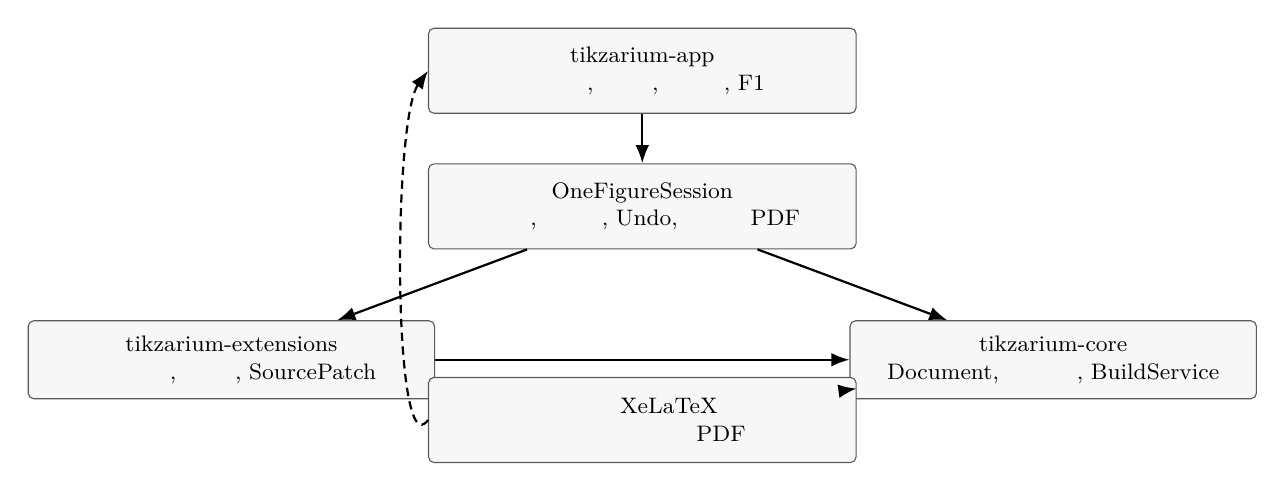
\begin{tikzpicture}[scale=0.90,transform shape,>=Latex,node distance=7mm and 9mm,font=\small,
  block/.style={draw=black!65,rounded corners=2pt,fill=black!3,text width=5.8cm,align=center,minimum height=12mm},
  smallblock/.style={draw=black!65,rounded corners=2pt,fill=black!3,text width=5.5cm,align=center,minimum height=11mm},
  arr/.style={->,thick}]
  \node[block] (ui) {tikzarium-app\\Один холст, исходник, инспектор, F1};
  \node[block,below=of ui] (session) {OneFigureSession\\Ревизия, выделение, Undo, состояние PDF};
  \node[smallblock,below left=10mm and -1mm of session] (adapter) {tikzarium-extensions\\Распознавание, свойства, SourcePatch};
  \node[smallblock,below right=10mm and -1mm of session] (core) {tikzarium-core\\Document, зависимости, BuildService};
  \node[block,below=18mm of session] (tex) {Внешний XeLaTeX\\Фактическая геометрия и PDF};
  \draw[arr] (ui)--(session);
  \draw[arr] (session)--(adapter);
  \draw[arr] (adapter.east)--(core.west);
  \draw[arr] (session)--(core);
  \draw[arr] (core)--(tex);
  \draw[arr,densely dashed] (tex.west) .. controls +(-0.5,-0.7) and +(-0.5,-0.7) .. (ui.west);
\end{tikzpicture}
\caption{Расширение существующих модулей. Пунктир обозначает возврат PDF.}
\end{figure}

\chapter{Архитектура расширений}\label{ux430ux440ux445ux438ux442ux435ux43aux442ux443ux440ux430-ux440ux430ux441ux448ux438ux440ux435ux43dux438ux439}

\section{OneFigureSession}\label{onefiguresession}

\texttt{OneFigureSession} --- новая внутренняя модель состояния. Она не заменяет существующий \texttt{Document}. Она хранит только выбранный рисунок, текущую ревизию, привязки распознанных команд и состояние сборки.

\begin{verbatim}
struct OneFigureSession {
    document: Document,
    revision: u64,
    selected: Option<InstanceId>,
    recognized: Vec<RecognizedInstance>,
    dependency_snapshot: ProjectDependencySnapshot,
    pending_build: Option<BuildEpoch>,
    preview_state: PreviewState,
}
\end{verbatim}

Представленная структура --- \textbf{проектируемый контракт}, а не готовый Rust API. Не создавайте второй источник текста. При ручной правке увеличьте ревизию. Удалите устаревшие экземпляры. Перестройте только нужные диапазоны распознавания.

\section{Контракт адаптера}\label{ux43aux43eux43dux442ux440ux430ux43aux442-ux430ux434ux430ux43fux442ux435ux440ux430}

Разделите распознавание, выдачу свойств и планирование правки. Планирование не должно изменять файл.

\begin{verbatim}
trait NativeTikzAdapter: Send + Sync {
    fn id(&self) -> &'static str;
    fn recognize(&self, source: &SourceView,
                 env: &FigureEnvironment) -> Vec<RecognizedInstance>;
    fn properties(&self, instance: &RecognizedInstance)
                  -> Vec<PropertyDescriptor>;
    fn plan_edit(&self, request: &EditRequest)
                 -> Result<SourcePatch, EditRefusal>;
    fn requirements(&self) -> AdapterRequirements;
}
\end{verbatim}

\texttt{SourceView} возвращает текст, ревизию, идентификатор файла и диапазоны безопасного разбора. \texttt{RecognizedInstance} возвращает ID адаптера, диапазон UTF-8, тип, свойства и точность распознавания. \texttt{EditRequest} содержит исходный диапазон, старое значение, новое значение и исходную ревизию. \texttt{SourcePatch} сохраняет контракт существующего продукта. При несовпадении значения или ревизии адаптер возвращает отказ.

\textbf{Запрет:} адаптер не вызывает XeLaTeX, не открывает сетевые соединения, не пишет файлов и не исправляет произвольный текст вокруг своей конструкции. Все действия записи проходят через одну проверяемую транзакцию.

\section{Алгоритм распознавания}\label{ux430ux43bux433ux43eux440ux438ux442ux43c-ux440ux430ux441ux43fux43eux437ux43dux430ux432ux430ux43dux438ux44f}

Реализуйте ограниченный лексический разбор. Он должен распознавать команды из явного перечня. Он не должен раскрывать произвольный TeX.

\begin{enumerate}
\def\labelenumi{\arabic{enumi}.}
\tightlist
\item
  Прочитайте неизменный снимок UTF-8.
\item
  Найдите известные команды: \texttt{\textbackslash{}draw}, \texttt{\textbackslash{}path}, \texttt{\textbackslash{}node}, \texttt{\textbackslash{}coordinate}, \texttt{\textbackslash{}begin\{axis\}}, \texttt{\textbackslash{}addplot}, \texttt{\textbackslash{}pic}, \texttt{\textbackslash{}dimline} и другие поддержанные конструкции.
\item
  Учитывайте сбалансированные группы \texttt{\{...\}} и \texttt{{[}...{]}}, экранированный \texttt{\%}, комментарии и математические группы.
\item
  Сохраните диапазон байтов каждой команды.
\item
  Определите простые литеральные ключи. Отдельно обозначьте выражения, имена координат и неопределённые макросы.
\item
  Передайте распознанный экземпляр одному специализированному адаптеру.
\item
  Верните \texttt{OPAQUE}, если синтаксис выходит за подтверждённую грамматику.
\end{enumerate}

Не допускайте скрытой нормализации пробелов и переносов строк. Не удаляйте комментарии в пользовательских файлах. Очищенные файлы Sarov служат только тестовыми образцами.

\section{Точечная правка}\label{ux442ux43eux447ux435ux447ux43dux430ux44f-ux43fux440ux430ux432ux43aux430}

Используйте существующие \texttt{SourceTarget} и \texttt{SourcePatch}. Вычисляйте кратчайший изменённый диапазон. Перед применением сравните старый текст и ревизию. При конфликте не вносите часть изменения.

\textbf{Пример:} пользователь изменил \texttt{samples=150} на \texttt{samples=180} в одном \texttt{\textbackslash{}addplot}. Измените только значение \texttt{150}. Не перестраивайте весь \texttt{axis}. Не переставляйте соседние ключи. Не раскрывайте пользовательскую функцию \texttt{gauss}.

\textbf{Проверка:} после одного действия Undo должен восстановить исходный SHA-256 файла. Все \texttt{.dat}, макросы и неизвестные блоки должны сохранить исходные SHA-256.

\section{Управление зависимостями}\label{ux443ux43fux440ux430ux432ux43bux435ux43dux438ux435-ux437ux430ux432ux438ux441ux438ux43cux43eux441ux442ux44fux43cux438}

Один активный рисунок может ссылаться на локальные данные. \texttt{AK-F6\_4} и \texttt{AK-F6\_5} подключают \texttt{optics-common.tex}. \texttt{AK-F14\_3}, \texttt{AK-F15\_1} и \texttt{AK-F21\_2} читают данные \texttt{plot\ file}. Это не другие активные рисунки.

Используйте существующие \texttt{BuildService} и \texttt{ProjectDependencySnapshot}. Отслеживайте исходник, локальные \texttt{.tex}, \texttt{.dat} и ресурсные файлы. Применяйте хэш каждого входа для определения актуальности PDF. Отдельно отмечайте зависимости TeX Live/MiKTeX, которые находятся вне корня проекта. Не объявляйте их локально проверенными.

\section{Состояния сборки}\label{ux441ux43eux441ux442ux43eux44fux43dux438ux44f-ux441ux431ux43eux440ux43aux438}

\begin{verbatim}
CLEAN_SOURCE → DIRTY_SOURCE → BUILDING → CURRENT_PDF
                     |            |         |
                     |            +→ FAILED | 
                     +→ STALE_PDF ←──────────┘
\end{verbatim}

После ошибки показывайте последний успешный PDF только со статусом «Устарел». Не выдавайте этот файл за результат новой компиляции. Параметры компилятора, предупреждения, версии пакетов и исходные ошибки сохраняйте для QA.

\section{Контракт версий каталога}\label{ux43aux43eux43dux442ux440ux430ux43aux442-ux432ux435ux440ux441ux438ux439-ux43aux430ux442ux430ux43bux43eux433ux430}

Не меняйте смысл текущих записей \texttt{catalog-v1.toml}. Добавьте внутреннее описание адаптеров с отдельной версией схемы. Не обещайте публичный стабильный ABI до испытаний двух независимых адаптеров. Зарегистрируйте, как минимум, \texttt{tikz.paths}, \texttt{pgfplots.axis}, \texttt{pgfplots.series}, \texttt{tikz.intersections}, \texttt{pgfplots.fillbetween}, \texttt{tikz.dimline}, \texttt{tikz.angles}, \texttt{tikz.math}.

Для каждого адаптера сохраните: точное имя команды, поддержанные ключи, типы и единицы, версию пакета, ограничения, синтаксис примера, метод правки, уровень распознавания, страницу справки. Не придумывайте значение по умолчанию. Указывайте \texttt{UNKNOWN}, если руководство его не подтверждает.

\chapter{Семейства адаптеров}\label{ux441ux435ux43cux435ux439ux441ux442ux432ux430-ux430ux434ux430ux43fux442ux435ux440ux43eux432}

\section{A. Базовая геометрия и путь}\label{a.-ux431ux430ux437ux43eux432ux430ux44f-ux433ux435ux43eux43cux435ux442ux440ux438ux44f-ux438-ux43fux443ux442ux44c}

\textbf{Назначение:} поддержать исходные команды TikZ, а не рисовать независимые объекты. Адаптер использует доступный набор команд \texttt{\textbackslash{}draw}, \texttt{\textbackslash{}path}, \texttt{\textbackslash{}fill}, \texttt{\textbackslash{}clip}, \texttt{\textbackslash{}node}, \texttt{\textbackslash{}coordinate}.

\textbf{Вход:} диапазон команды и стиль на момент распознавания. \textbf{Свойства:} цвет, толщина линии, штриховка, наконечник, видимость, координата, размер, anchor. \textbf{Выход:} план точечной правки или обоснованный отказ.

Разделите простые и вычисляемые координаты. Для пары литералов \texttt{(2,3)} можно изменить числовой компонент. Для \texttt{(\$(A)!0.5!(B)\$)} разрешите только документированную правку исходного коэффициента. Не вычисляйте экранный результат в Rust как авторитетную координату.

Отдельно распознавайте \texttt{-\/-}, \texttt{..\ controls\ ...\ ..}, \texttt{rectangle}, \texttt{circle}, \texttt{ellipse}, \texttt{arc}, \texttt{cycle}, \texttt{++}, \texttt{+(...)}, ключи \texttt{shift}, \texttt{rotate}, \texttt{scale}. Если путь содержит неизвестный макрос, не изменяйте геометрию этого участка визуальным перетаскиванием.

\textbf{Приёмка:} базовые шесть инструментов продолжают проходить прежние тесты N1. Дополнительно проверены arcs/ellipse, относительные координаты, области scope и сохранение порядка операций. Испытания применяют настоящие исходные команды, а не копирование текста в буфер.

\section{B. PGFPlots: оси и ряды}\label{b.-pgfplots-ux43eux441ux438-ux438-ux440ux44fux434ux44b}

\textbf{Назначение:} пользователь изменяет существующий график через свойства. PGFPlots строит форму графика в PDF.

\textbf{Модель:} распознанный \texttt{axis} содержит локальные серии \texttt{\textbackslash{}addplot} и ссылки на имена путей. Не храните вторую независимую таблицу точек, которая стала бы источником истины. Серия хранит только ссылку на исходный диапазон и параметры, которые можно доказанно изменить.

\textbf{Поддержка первого вертикального сценария:} \texttt{\textbackslash{}begin\{axis\}{[}...{]}}, \texttt{\textbackslash{}addplot{[}...{]}\{...\}}, \texttt{domain}, \texttt{samples}, \texttt{xmin/xmax}, \texttt{ymin/ymax}, \texttt{width}, \texttt{height}, \texttt{mark}, \texttt{line\ width}, \texttt{color}, \texttt{xlabel}, \texttt{ylabel}, \texttt{xtick}, \texttt{ytick}, \texttt{clip}. Сохраните \texttt{\textbackslash{}pgfplotsset\{compat=1.17\}} из Sarov. При неизвестной версии пакета оставьте статус проверки неопределённым.

\textbf{Поддержка второго сценария:} несколько серий с независимыми формулами. При изменении одной серии сохраните остальные серии, их порядок и связанные имена \texttt{name\ path}. Не переписывайте серию целиком, если пользователь изменил только \texttt{domain}.

\textbf{Поддержка третьего сценария:} \texttt{plot\ coordinates} и числовые таблицы. Не округляйте входные значения. Если точка содержит выражение или макрос, покажите его в свойствах как исходный текст.

\textbf{Отдельная особенность:} нативный TikZ \texttt{plot\ (\textbackslash{}x,\{...\})} не является \texttt{\textbackslash{}addplot}. Используйте два разных адаптера. Оба используют PGF Math для вычислений. \texttt{SV-040} не должен запускать внешний вычислитель.

\textbf{Приёмка:} \texttt{SV-001}, \texttt{SV-003}, \texttt{SV-009}, \texttt{SV-022}, \texttt{SV-029}, \texttt{SV-040}, \texttt{SV-042}. Для каждого примера выполните правку ключа, PDF и возврат исходного SHA-256.

\section{C. Именованные пути, пересечения и заливки}\label{c.-ux438ux43cux435ux43dux43eux432ux430ux43dux43dux44bux435-ux43fux443ux442ux438-ux43fux435ux440ux435ux441ux435ux447ux435ux43dux438ux44f-ux438-ux437ux430ux43bux438ux432ux43aux438}

\textbf{Назначение:} сохранить ссылки между объектами. Путь с \texttt{name\ path=A} может использоваться в другой команде. Пересечение \texttt{intersection-1} зависит от этих путей. Заливка \texttt{fill\ between} также зависит от двух именованных кривых.

Не изменяйте вычисленную точку пересечения как свободную экранную координату. Предоставьте редактирование исходных путей и параметров вычисления. После правки запустите XeLaTeX. При изменении имени пути обновляйте ссылки только через отдельную проверенную транзакцию; до появления такого адаптера сделайте поле имени доступным только для чтения.

Порядок слоёв, \texttt{soft\ clip}, \texttt{\textbackslash{}clip}, \texttt{patterns} и \texttt{patterns.meta} влияет на результат. Сохраняйте исходный порядок операций. Не переносите заливку в другой слой для упрощения GUI. Не превращайте паттерн в растровую текстуру.

\textbf{Приёмка:} \texttt{SV-006}, \texttt{SV-007}, \texttt{SV-010}, \texttt{SV-027}, \texttt{SV-028}, \texttt{SV-039}. Проверьте названия путей, пересечения и ограничения заливки. При отсутствии доказанной связи адаптер обязан вернуть \texttt{OPAQUE}.

\section{D. Углы, размерные линии и формы}\label{d.-ux443ux433ux43bux44b-ux440ux430ux437ux43cux435ux440ux43dux44bux435-ux43bux438ux43dux438ux438-ux438-ux444ux43eux440ux43cux44b}

Адаптер \texttt{angles} изменяет параметры \texttt{\textbackslash{}pic} и сохраняет ссылки на исходные вершины. Адаптер \texttt{tikz-dimline} изменяет размерные линии. Сохраните крайние точки, выносные линии, наконечники и положение подписи. Не создавайте визуально похожую произвольную стрелку вместо размерной линии.

Адаптеры \texttt{shapes.geometric} и \texttt{shapes.arrows} должны сохранять имя формы, свойства узла и anchors. Если форма из пакета не поддержана, показывайте PDF и исходник, но не выдавайте ложные управляющие маркеры.

\textbf{Приёмка:} \texttt{SV-005}, \texttt{SV-035}, \texttt{SV-036}, \texttt{SV-038}. Проверка включает F1, доступность свойства, SourcePatch, PDF и Undo.

\section{E. Макросы, циклы и PGF Math}\label{e.-ux43cux430ux43aux440ux43eux441ux44b-ux446ux438ux43aux43bux44b-ux438-pgf-math}

Сохраняйте определения \texttt{\textbackslash{}def}, \texttt{\textbackslash{}newcommand}, \texttt{\textbackslash{}pgfmathsetmacro}, \texttt{\textbackslash{}pgfmathdeclarefunction}, \texttt{\textbackslash{}tikzset} без принудительного раскрытия. Интерфейс может разрешить изменение известного литерального аргумента. Он не должен изменять результат вычисления через запись новой координаты.

Для простого \texttt{\textbackslash{}foreach} поддержите переменную цикла и литеральный список. Не разворачивайте цикл в множество самостоятельных команд. Вложенные циклы и вычисляемые множества могут оставаться доступными только в исходнике.

Для оптических схем \texttt{AK-F6\_4} и \texttt{AK-F6\_5} допускайте изменение входного параметра макроса. Пересчёт геометрии выполняет TeX. Обновляйте карту зависимостей, если параметр расположен в подключённом \texttt{optics-common.tex}.

\textbf{Приёмка:} \texttt{AK-F3\_1}, \texttt{AK-F6\_4}, \texttt{AK-F6\_5}, \texttt{SV-042}, выбранные рисунки с \texttt{\textbackslash{}foreach}. Нельзя получить PASS, если редактировалась экранная координата вместо формулы источника.

\section{F. Данные, шрифты и публикационное качество}\label{f.-ux434ux430ux43dux43dux44bux435-ux448ux440ux438ux444ux442ux44b-ux438-ux43fux443ux431ux43bux438ux43aux430ux446ux438ux43eux43dux43dux43eux435-ux43aux430ux447ux435ux441ux442ux432ux43e}

Проверяйте существование и хэш всех локальных \texttt{.dat}. Не изменяйте точки файла данных при редактировании стиля. Сборка должна повторяться при изменении зависимости. Для одной активной фигуры используйте один снимок входных ресурсов. Подключаемые исходники могут быть открыты в текстовом редакторе для диагностики, но не должны становиться вторым активным холстом.

В документах используются \texttt{fontspec}, \texttt{unicode-math}, \texttt{polyglossia}, \texttt{Noto\ Sans}, \texttt{Noto\ Serif}, \texttt{STIX\ Two\ Math}, \texttt{Charis\ SIL}. Не включайте лицензионные файлы шрифтов в поставку. Определяйте доступность локально. Сборка с кодом 0 не гарантирует наличие всех глифов. Отдельно проверяйте \texttt{Missing\ character}, \texttt{pdffonts}, читаемость русских подписей и математических символов.

В актуальной проверке Linux зафиксированы 120 предупреждений \texttt{nullfont} в 13 Sarov-рисунках. Тесты должны хранить эти предупреждения. Разделите проверку шрифтов и сборку PDF.

\chapter{Формальные технические требования}\label{ux444ux43eux440ux43cux430ux43bux44cux43dux44bux435-ux442ux435ux445ux43dux438ux447ux435ux441ux43aux438ux435-ux442ux440ux435ux431ux43eux432ux430ux43dux438ux44f}

Каждое требование имеет постоянный идентификатор. Изменение требования требует новой версии ТЗ. Критерий приёмки задаёт наблюдаемый результат. Таблица ниже является нормативной частью документа. Файл \texttt{REQUIREMENTS.csv} содержит те же записи для автоматизированной проверки и планирования.


\clearpage
\begin{longtable}{@{}>{\raggedright\arraybackslash}p{2.35cm}>{\raggedright\arraybackslash}p{0.75cm}>{\raggedright\arraybackslash}p{6.35cm}>{\raggedright\arraybackslash}p{5.2cm}@{}}
\caption{Нормативные требования Scientific-142} \\

\toprule
\textbf{ID} & \textbf{P} & \textbf{Требование} & \textbf{Проверка} \\ \midrule
\endfirsthead
\multicolumn{4}{@{}l}{\small Продолжение таблицы требований} \\ \midrule
\textbf{ID} & \textbf{P} & \textbf{Требование} & \textbf{Проверка} \\ \midrule
\endhead
\midrule \multicolumn{4}{r}{\footnotesize Продолжение на следующей странице} \\ \endfoot
\bottomrule \endlastfoot
\footnotesize SC-SCOPE-001 & P0 & Редактор открывает один активный рисунок. Редактор не создаёт галерею рисунков. & Один файл, один холст, один PDF. Тест SC-UI-001. \\ \addlinespace[2pt]
\footnotesize SC-SCOPE-002 & P0 & Программа хранит обычный UTF-8 .tex или .tikz. Программа не вводит обязательный собственный формат. & Save/Open сохраняют исходник. Тест SC-SOURCE-001. \\ \addlinespace[2pt]
\footnotesize SC-SCOPE-003 & P0 & Рядом с холстом постоянно доступен редактируемый исходный текст. & Выбор инструмента показывает соответствующую команду. \\ \addlinespace[2pt]
\footnotesize SC-SCOPE-004 & P0 & Один рисунок может содержать локальные .dat и подключаемые .tex. Эти файлы не становятся другими активными рисунками. & AK-F6\_4 и AK-F14\_3 открываются как один рисунок. \\ \addlinespace[2pt]
\footnotesize SC-SCOPE-005 & P0 & Сводный Sarov main.tex не является входным форматом пользовательского мультиредактора. & Каждый SV-001...SV-042 открывается отдельно. \\ \addlinespace[2pt]
\footnotesize SC-SCOPE-006 & P0 & Gnuplot не входит в поставку, обнаружение зависимостей и план адаптеров. & SV-040 собирается без shell escape и Gnuplot. \\ \addlinespace[2pt]
\footnotesize SC-SRC-001 & P0 & Распознаватель возвращает диапазон байтов UTF-8 и ревизию документа для каждой поддерживаемой конструкции. & Выбранная команда показывает точный диапазон исходника. \\ \addlinespace[2pt]
\footnotesize SC-SRC-002 & P0 & Распознаватель различает литерал, вычисляемое выражение и неизвестную конструкцию. & Неизвестная конструкция имеет статус OPAQUE. \\ \addlinespace[2pt]
\footnotesize SC-SRC-003 & P0 & Распознаватель учитывает вложенные фигурные и квадратные скобки, строковые проценты и комментарии. & Тесты сбалансированных параметров не меняют соседний код. \\ \addlinespace[2pt]
\footnotesize SC-SRC-004 & P0 & Распознаватель не выполняет произвольные пользовательские макросы. & Макрос с неизвестным результатом остаётся OPAQUE. \\ \addlinespace[2pt]
\footnotesize SC-SRC-005 & P0 & Система сохраняет идентификатор владения диапазоном и не изменяет соседние команды. & Патч затрагивает только подтверждённый диапазон. \\ \addlinespace[2pt]
\footnotesize SC-SRC-006 & P0 & Планировщик правки передаёт SourcePatch с проверкой старого текста и ревизии. & Правка при устаревшей ревизии отклоняется. \\ \addlinespace[2pt]
\footnotesize SC-SRC-007 & P0 & После ручного изменения исходника программа аннулирует устаревшие маркеры и выполняет повторное распознавание. & Параметры не применяются к прежним диапазонам. \\ \addlinespace[2pt]
\footnotesize SC-SRC-008 & P0 & Одна операция инспектора создаёт одну операцию Undo. & Undo восстанавливает исходный SHA-256. \\ \addlinespace[2pt]
\footnotesize SC-SRC-009 & P0 & Программа сохраняет неизвестные команды, комментарии, пробелы и CRLF пользовательского исходника. & Неизменённые байты совпадают до и после правки. \\ \addlinespace[2pt]
\footnotesize SC-SRC-010 & P0 & Сохранение исходника происходит атомарно с обработкой ошибок записи. & При отказе записи прежний файл остаётся целым. \\ \addlinespace[2pt]
\footnotesize SC-SRC-011 & P0 & Планировщик отклоняет правку при перекрывающихся диапазонах владения. & Нет частично применённого изменения. \\ \addlinespace[2pt]
\footnotesize SC-SRC-012 & P1 & Инспектор показывает обоснование отказа без автоматической замены числовой геометрией. & Ошибка OPAQUE указывает на редактирование кода. \\ \addlinespace[2pt]
\footnotesize SC-UI-001 & P0 & Рабочая область показывает холст, исходник, свойства и точный PDF одного рисунка. & Проверка при 1366×768 и масштабе 100/125/200 \%. \\ \addlinespace[2pt]
\footnotesize SC-UI-002 & P0 & Выбор элемента подсвечивает его исходную команду. & Подсветка соответствует байтовому диапазону. \\ \addlinespace[2pt]
\footnotesize SC-UI-003 & P0 & Инспектор использует общий каталог команд и параметров. & Справка и параметры одного ключа не противоречат друг другу. \\ \addlinespace[2pt]
\footnotesize SC-UI-004 & P0 & Точное изображение строит внешний XeLaTeX. Холст показывает только предварительные маркеры. & Границы предварительного слоя визуально различимы. \\ \addlinespace[2pt]
\footnotesize SC-UI-005 & P0 & Редактор показывает статус текущего PDF: актуален, устарел или ошибка. & После ошибки экспорт старого PDF не обозначается как новый. \\ \addlinespace[2pt]
\footnotesize SC-UI-006 & P0 & Пользователь может открыть F1 по ключу и увидеть синтаксис, эффект, ограничения и ссылку на руководство. & Для каждого нового элемента каталога есть одна карточка справки. \\ \addlinespace[2pt]
\footnotesize SC-UI-007 & P1 & Редактор показывает зависимости рисунка и ошибки поиска ресурсов. & Прямые .dat и \textbackslash{}input показаны с путями. \\ \addlinespace[2pt]
\footnotesize SC-UI-008 & P1 & Угол и размерная линия имеют специализированный инспектор. & SV-005 и SV-035 изменяются через соответствующие параметры. \\ \addlinespace[2pt]
\footnotesize SC-PATH-001 & P0 & Адаптер path поддерживает draw, path, fill, clip и общие стилевые ключи, если синтаксис распознан. & Изменение line width не меняет точки пути. \\ \addlinespace[2pt]
\footnotesize SC-PATH-002 & P0 & Адаптер поддерживает прямые, стрелки, прямоугольники, окружности и кубические кривые Безье. & Существующие шесть примитивов не регрессируют. \\ \addlinespace[2pt]
\footnotesize SC-PATH-003 & P0 & Адаптер распознаёт arc, ellipse, cycle и замыкание пути. & Редактирование параметра не удаляет cycle. \\ \addlinespace[2pt]
\footnotesize SC-PATH-004 & P0 & Адаптер сохраняет относительные координаты и путь ++ без замены на абсолютные числа. & Синтаксис исходника остаётся относительным. \\ \addlinespace[2pt]
\footnotesize SC-PATH-005 & P0 & Адаптер calc изменяет только подтверждённый входной литерал. & Связанные узлы пересчитывает XeLaTeX. \\ \addlinespace[2pt]
\footnotesize SC-PATH-006 & P0 & Адаптер различает scope и локальные преобразования shift, rotate, scale. & Правка не переносит команду в другую область действия. \\ \addlinespace[2pt]
\footnotesize SC-PATH-007 & P0 & Адаптер сохраняет порядок наложения path, fill и draw. & Порядок исходных команд не изменяется. \\ \addlinespace[2pt]
\footnotesize SC-PATH-008 & P1 & Адаптер узлов поддерживает anchor, text, font, inner sep и позиционирование. & Русский текст и TeX-формулы остаются без преобразований. \\ \addlinespace[2pt]
\footnotesize SC-PATH-009 & P1 & Адаптер позволяет изменять точный размер наконечника из arrows.meta. & SV и AK сохраняют геометрию концов стрелок. \\ \addlinespace[2pt]
\footnotesize SC-PATH-010 & P1 & Адаптер поддерживает повторяющиеся стили через тикзset без разворачивания определения. & Правка общего стиля не заменяет отдельные команды. \\ \addlinespace[2pt]
\footnotesize SC-PLOT-001 & P0 & PGFPlots-адаптер распознаёт окружение axis и связанные с ним plot серии. & SV-001 показывает один axis и одну серию. \\ \addlinespace[2pt]
\footnotesize SC-PLOT-002 & P0 & Адаптер сохраняет \textbackslash{}pgfplotsset\{compat=1.17\} и пользовательский профиль совместимости. & Компиляция не изменяет compat. \\ \addlinespace[2pt]
\footnotesize SC-PLOT-003 & P0 & Адаптер изменяет ключи axis: xmin, xmax, ymin, ymax, width, height. & Изменение одного ключа создаёт минимальный SourcePatch. \\ \addlinespace[2pt]
\footnotesize SC-PLOT-004 & P0 & Адаптер изменяет ticks, ticklabels, xlabel, ylabel и расположение осей. & SV-001/003 после правки имеют читаемый PDF. \\ \addlinespace[2pt]
\footnotesize SC-PLOT-005 & P0 & Адаптер распознаёт \textbackslash{}addplot и \textbackslash{}addplot+ с формульной серией. & Выбор серии подсвечивает исходный addplot. \\ \addlinespace[2pt]
\footnotesize SC-PLOT-006 & P0 & Адаптер изменяет literal domain, samples, line width, color и mark. & Правка и Undo проходят на SV-001 и SV-029. \\ \addlinespace[2pt]
\footnotesize SC-PLOT-007 & P0 & Адаптер поддерживает plot coordinates без перестановки точек. & Число и порядок точек неизменны. \\ \addlinespace[2pt]
\footnotesize SC-PLOT-008 & P0 & Адаптер распознаёт нативный TikZ plot по функции PGF Math. & SV-040 строится без Gnuplot. \\ \addlinespace[2pt]
\footnotesize SC-PLOT-009 & P0 & Адаптер сохраняет математическую формулу как исходный TeX, не оценивая её в Rust. & Неизвестный аргумент не преобразуется в приближение. \\ \addlinespace[2pt]
\footnotesize SC-PLOT-010 & P0 & Адаптер не изменяет неизвестные plot options и пользовательские pgfkeys. & Сохранены все исходные неизвестные ключи. \\ \addlinespace[2pt]
\footnotesize SC-PLOT-011 & P1 & Адаптер распознаёт legend и named plot path, не меняя их при правке других свойств. & Легенда и имя пути сохранены. \\ \addlinespace[2pt]
\footnotesize SC-PLOT-012 & P1 & Система ограничивает затраты UI на серии с тысячами точек. & Прокрутка интерфейса не блокируется повторной обработкой всех координат. \\ \addlinespace[2pt]
\footnotesize SC-GEO-001 & P0 & Адаптер распознаёт имя пути name path. & Пользователь видит установленное имя. \\ \addlinespace[2pt]
\footnotesize SC-GEO-002 & P0 & Адаптер поддерживает name intersections и ссылки intersection-N. & После изменения исходного пути пересечение пересчитывает XeLaTeX. \\ \addlinespace[2pt]
\footnotesize SC-GEO-003 & P0 & Адаптер не записывает координаты пересечения из экранных пикселей. & Непрозрачное пересечение имеет статус OPAQUE. \\ \addlinespace[2pt]
\footnotesize SC-GEO-004 & P0 & Адаптер fill between сохраняет имена двух исходных серий. & SV-006/027 не теряют привязку к путям. \\ \addlinespace[2pt]
\footnotesize SC-GEO-005 & P0 & Адаптер поддерживает soft clip и параметры заливки между кривыми. & Участок заливки после правки вычисляет PGFPlots. \\ \addlinespace[2pt]
\footnotesize SC-GEO-006 & P1 & Адаптер позволяет изменять patterns и patterns.meta без изменения контура. & Свойства заливки меняются отдельно от геометрии. \\ \addlinespace[2pt]
\footnotesize SC-GEO-007 & P1 & Адаптер учитывает pgf layers и clip при построении предварительного слоя. & Нельзя ошибочно выделить скрытую фигуру как видимую. \\ \addlinespace[2pt]
\footnotesize SC-GEO-008 & P1 & Адаптер angle pic сохраняет ссылки на три исходные точки. & SV-038 изменяет радиус дуги без смещения точек. \\ \addlinespace[2pt]
\footnotesize SC-GEO-009 & P1 & Адаптер tikz-dimline сохраняет выносные линии и подпись измерения. & Размерная линия меняется только в разрешённом диапазоне. \\ \addlinespace[2pt]
\footnotesize SC-GEO-010 & P1 & Адаптер shapes.geometric и shapes.arrows сохраняет исходные виды узлов. & SV-035/036 не заменяются растровым объектом. \\ \addlinespace[2pt]
\footnotesize SC-MATH-001 & P0 & Адаптер различает \textbackslash{}def, \textbackslash{}newcommand и \textbackslash{}pgfmathsetmacro как объявления, а не вычисленные значения. & Редактор не изменяет раскрытый результат вместо определения. \\ \addlinespace[2pt]
\footnotesize SC-MATH-002 & P0 & Адаптер распознаёт \textbackslash{}pgfmathdeclarefunction и число параметров. & SV-042 показывает gauss/3 в каталоге параметров. \\ \addlinespace[2pt]
\footnotesize SC-MATH-003 & P0 & Редактор меняет известный literal аргумент без разворачивания PGF Math. & SV-042 сохраняет две формулы гауссиан. \\ \addlinespace[2pt]
\footnotesize SC-MATH-004 & P1 & Адаптер \textbackslash{}foreach распознаёт простой литеральный диапазон и переменную цикла. & Пользователь меняет диапазон, но не результат раскрытия. \\ \addlinespace[2pt]
\footnotesize SC-MATH-005 & P1 & Неподдерживаемые вложенные циклы остаются доступными в исходнике. & Распознаватель не пытается записать все развёрнутые узлы. \\ \addlinespace[2pt]
\footnotesize SC-MATH-006 & P0 & Адаптер сохраняет математические инварианты, если сценарий имеет явную проверку. & Для AK-F3\_3 сохраняется интеграл нулевой площади. \\ \addlinespace[2pt]
\footnotesize SC-MATH-007 & P0 & Непроверенное физическое свойство нельзя объявлять доказанным. & L4 статус отделён от L1 и L3. \\ \addlinespace[2pt]
\footnotesize SC-DATA-001 & P0 & Система собирает локальный граф входных ресурсов из \textbackslash{}input, plot file и .fls. & AK-F6\_4 и AK-F14\_3 имеют полный список зависимостей. \\ \addlinespace[2pt]
\footnotesize SC-DATA-002 & P0 & Путь ресурса разрешается относительно файла и корня проекта. & Отсутствие данных выдаёт понятную ошибку. \\ \addlinespace[2pt]
\footnotesize SC-DATA-003 & P0 & Повторная сборка выполняется при изменении ресурса. & Правка .dat переводит текущий PDF в статус устарел. \\ \addlinespace[2pt]
\footnotesize SC-DATA-004 & P0 & Операция редактирования холста не изменяет данные plot file. & SHA каждого .dat остаётся прежним. \\ \addlinespace[2pt]
\footnotesize SC-DATA-005 & P1 & Система показывает, из какого файла получена ошибка TeX. & Переход к диагностике открывает правильный файл. \\ \addlinespace[2pt]
\footnotesize SC-DATA-006 & P1 & Непрозрачная условная загрузка файла получает статус UNKNOWN. & Система не присваивает ложно подтверждённый путь. \\ \addlinespace[2pt]
\footnotesize SC-DATA-007 & P0 & Система не использует символические ссылки для выхода из доверенного корня без явного разрешения. & Реестр зависимостей отмечает внешний путь. \\ \addlinespace[2pt]
\footnotesize SC-PKG-001 & P0 & Система различает установку пакета, подключение в проекте, совместимость движка, поддержку GUI и наличие справки. & Пять статусов выводятся отдельно. \\ \addlinespace[2pt]
\footnotesize SC-PKG-002 & P0 & Подключение пакета создаёт видимый SourcePatch, но не устанавливает пакет. & Дифф можно отменить. \\ \addlinespace[2pt]
\footnotesize SC-PKG-003 & P0 & Адаптер содержит версионированные сведения о синтаксисе и документации. & F1 указывает оригинальные команды и руководство. \\ \addlinespace[2pt]
\footnotesize SC-PKG-004 & P0 & Каталог поддерживает PGFPlots и tikz-dimline как независимые семейства. & Наличие .sty не означает GUI PASS. \\ \addlinespace[2pt]
\footnotesize SC-PKG-005 & P1 & Новый каталог не меняет семантику существующих шести примитивов. & Прежние unit tests N1/N2/N3 проходят без изменений. \\ \addlinespace[2pt]
\footnotesize SC-PKG-006 & P0 & Внешние декларативные манифесты не исполняют код, процессы и сетевые запросы. & Нет динамического DLL/dylib подключения. \\ \addlinespace[2pt]
\footnotesize SC-BUILD-001 & P0 & Сборщик вызывает установленный пользователем XeLaTeX без оболочки. & Команда и аргументы сохранены в доказательстве. \\ \addlinespace[2pt]
\footnotesize SC-BUILD-002 & P0 & Сборщик отключает shell escape по умолчанию. & Ни один fixture не требует Gnuplot. \\ \addlinespace[2pt]
\footnotesize SC-BUILD-003 & P0 & MiKTeX использует режим без автоматической установки пакетов. & Тест Windows не изменяет глобальные настройки MiKTeX. \\ \addlinespace[2pt]
\footnotesize SC-BUILD-004 & P0 & Сборщик ограничивает время задачи и поддерживает отмену. & Отмена не блокирует интерфейс. \\ \addlinespace[2pt]
\footnotesize SC-BUILD-005 & P0 & Система не использует отсутствие ошибки как доказательство полной отрисовки. & Отдельно проверены PDF, страницы, шрифты и изображение. \\ \addlinespace[2pt]
\footnotesize SC-BUILD-006 & P0 & После ошибки программа хранит последний успешный PDF только как устаревший. & Устаревший PDF не получает статус текущего результата. \\ \addlinespace[2pt]
\footnotesize SC-BUILD-007 & P1 & Система проверяет встраивание шрифтов и отсутствие пропущенных символов. & 120 предупреждений nullfont сохраняются в отчёте QA. \\ \addlinespace[2pt]
\footnotesize SC-BUILD-008 & P0 & Запуск под существующим Administrator допускается с предупреждением о доверенных документах. & Не требуется новый пользователь или изменение UAC. \\ \addlinespace[2pt]
\footnotesize SC-BUILD-009 & P0 & Сборка не изменяет исходники и локальные зависимости рисунка. & SHA всех входных файлов совпадает до и после. \\ \addlinespace[2pt]
\footnotesize SC-QA-001 & P0 & Реестр содержит 142 уникальных идентификатора и SHA-256 исходников. & 100 AK и 42 SR подтверждены валидатором. \\ \addlinespace[2pt]
\footnotesize SC-QA-002 & P0 & Каждый тестовый исходник содержит одно активное окружение tikzpicture. & Валидатор отклоняет неправильную структуру. \\ \addlinespace[2pt]
\footnotesize SC-QA-003 & P0 & Сценарий L1 проверяет фактический запуск XeLaTeX и одностраничный PDF. & Файл compile-evidence.csv содержит 142 результата. \\ \addlinespace[2pt]
\footnotesize SC-QA-004 & P0 & Сценарий L2 проверяет распознавание поддерживаемой конструкции и её диапазона. & Тест использует production recognizer, не независимый парсер. \\ \addlinespace[2pt]
\footnotesize SC-QA-005 & P0 & Сценарий L3 проверяет реальный GUI edit, SourcePatch, PDF, Undo и сохранность соседнего кода. & Для каждого рисунка требуется отдельное доказательство. \\ \addlinespace[2pt]
\footnotesize SC-QA-006 & P0 & Сценарий L4 проверяет физический инвариант только там, где имеется формальное правило. & Непроверенные формулы остаются NOT\_RUN. \\ \addlinespace[2pt]
\footnotesize SC-QA-007 & P0 & Хэш эталонного PDF сохраняется независимо от хэша новой сборки. & Различие PDF не скрывается под общим PASS. \\ \addlinespace[2pt]
\footnotesize SC-QA-008 & P0 & Сравнение растров выполняется на зафиксированном окружении и с указанием порога. & Статус сравнения отделён от статуса компиляции. \\ \addlinespace[2pt]
\footnotesize SC-QA-009 & P0 & Негативный тест изменённого fixture обязан завершиться отказом. & Манифест отвергает повреждение SHA. \\ \addlinespace[2pt]
\footnotesize SC-QA-010 & P0 & Hosted CI, Windows Server и физическая Windows 10 имеют разные статусы. & Не допускается перенос PASS между платформами. \\ \addlinespace[2pt]
\footnotesize SC-QA-011 & P1 & QA хранит исходные PDF, логи, SHA и параметры окружения. & Результат можно повторить по инструкции. \\ \addlinespace[2pt]
\footnotesize SC-QA-012 & P1 & Статус каждой возможности определяется отдельно для L0...L4. & Нельзя повышать L3 по успешной компиляции L1. \\ \addlinespace[2pt]
\footnotesize SC-PERF-001 & P1 & Распознаватель не блокирует поток UI на больших plot coordinates. & Интерактивный ответ остаётся отзывчивым на тяжёлой фигуре. \\ \addlinespace[2pt]
\footnotesize SC-PERF-002 & P1 & Кэш ключуется хэшами источника, ресурсов, движка и версии пакетов. & При изменении .dat PDF помечается устаревшим. \\ \addlinespace[2pt]
\footnotesize SC-PERF-003 & P1 & Размер журналов и выходных файлов ограничивается. & При превышении лимита выводится отдельная диагностика. \\ \addlinespace[2pt]
\footnotesize SC-PERF-004 & P1 & Пользователь отменяет длительную сборку без потери исходника. & Незавершённый процесс завершается и файлы сохранены. \\ \addlinespace[2pt]
\end{longtable}
\normalsize


\chapter{Комплект входных испытаний}\label{ux43aux43eux43cux43fux43bux435ux43aux442-ux432ux445ux43eux434ux43dux44bux445-ux438ux441ux43fux44bux442ux430ux43dux438ux439}

\section{Структура файлов}\label{ux441ux442ux440ux443ux43aux442ux443ux440ux430-ux444ux430ux439ux43bux43eux432}

Комплект содержит ровно 142 независимых входных \texttt{.tex}. Каждая активная фигура имеет один \texttt{\textbackslash{}begin\{tikzpicture\}} и один \texttt{\textbackslash{}end\{tikzpicture\}}. Данные и общие макросы размещены рядом с тестами. Никакая тестовая фигура не требует подключения другого активного рисунка.

\begin{verbatim}
SCIENTIFIC-142/
  docs/
    SCIENTIFIC_142_TRD_R4.tex
    SCIENTIFIC_142_TRD_R4.pdf
  fixtures/
    AK/
      data/                         74 локальных файла .dat
      F3_1/figure.tex
      ...                           всего 100 рисунков
      F6_4/optics-common.tex       общая геометрия
      F6_5/optics-common.tex
    SR/
      SV-001/figure.tex
      ...
      SV-042/figure.tex           42 подготовленных рисунка
  references/
    AK/*.pdf                       100 эталонных PDF
    SR/*.pdf                       42 эталонных PDF
  provenance/
    Sarov_main_original.tex        неизменённый переданный источник
    SOURCES_SHA256.txt
  qa/
    validate_corpus.py
    compile_suite.py
    compare_reference.py
    test_negative.py
    GUI_SCENARIOS.jsonl
  evidence/
    compile-evidence.csv
    summary.json
    raster-evidence.csv
    raster-summary.json
  QA_MANIFEST.json
  QA_MATRIX.csv
  REQUIREMENTS.csv
\end{verbatim}

Комплект не распространяет файлы шрифтов или TeX Live/MiKTeX. Они являются внешними предпосылками. Самодостаточность означает наличие \textbf{всех локальных источников, данных, макросов, эталонов, инструментов проверки и описания требований}.

\section{Происхождение AK-100}\label{ux43fux440ux43eux438ux441ux445ux43eux436ux434ux435ux43dux438ux435-ak-100}

AK-100 взят из неизменённого итогового комплекта 7 ноября 2026 года. Тестовые исходники скопированы побайтово. Не изменены авторские математические формулы, комментарии, пробелы и стили. Программа должна уметь сохранять такие комментарии при обычном редактировании.

Для некоторых рисунков \texttt{\textbackslash{}datadir} ссылается на \texttt{../data}. Поэтому runner выполняет TeX из папки конкретного рисунка. Общий каталог \texttt{fixtures/AK/data} содержит 74 исходных \texttt{.dat}. Для \texttt{AK-F6\_4} и \texttt{AK-F6\_5} рядом с исходником находится \texttt{optics-common.tex}. Эталонные PDF хранятся независимо от новой сборки.

\section{Происхождение Sarov-42}\label{ux43fux440ux43eux438ux441ux445ux43eux436ux434ux435ux43dux438ux435-sarov-42}

Sarov-42 подготовлен из \texttt{Sarov\_pics\ {[}TikZ{]}.zip/main.tex}. Подготовка извлекла 42 действующих окружения TikZ в 42 самостоятельных файла. В тестовых копиях удалены комментарии. Исходный \texttt{main.tex} сохранён для проверки происхождения и не используется как рабочий документ Tikzarium.

Два теста содержат документированные исправления исходной ошибки или внешней зависимости:

\begin{itemize}
\tightlist
\item
  \texttt{SV-040}: формула кривой использует штатный PGF Math вместо Gnuplot.
\item
  \texttt{SV-042}: два ошибочных вызова \texttt{\textbackslash{}gauss} заменены вызовами объявленной PGF Math функции.
\end{itemize}

Тестовые файлы --- подготовленные образы. Они не являются побайтовыми копиями всех строк \texttt{main.tex}. Манифест хранит исходный и подготовленный SHA-256 отдельно.

\section{Машинный манифест}\label{ux43cux430ux448ux438ux43dux43dux44bux439-ux43cux430ux43dux438ux444ux435ux441ux442}

\texttt{QA\_MANIFEST.json} содержит для каждого объекта: ID, корпус, относительный путь, SHA-256 исходника, эталонный PDF и его SHA-256, локальные зависимости, заявленные пакеты, заявленные библиотеки, обнаруженные конструкции и нормализации. Поле \texttt{source\_kind} различает исходный файл и подготовленную QA-копию.

\texttt{QA\_MATRIX.csv} содержит уровни L0--L4. CSV имеет кодировку UTF-8 с BOM и разделитель \texttt{;}. Разделители и кавычки обработаны стандартным CSV-писателем. Не считайте значения \texttt{PENDING} или \texttt{NOT\_RUN} успешными проверками.

\texttt{qa/GUI\_SCENARIOS.jsonl} содержит 142 будущих сценария для настоящего интерфейса. Эти сценарии имеют статус \texttt{NOT\_RUN}. Они задают требуемое действие и контрольные условия. Они не утверждают, что GUI уже реализовал нужный адаптер.

\section{Запуск проверок}\label{ux437ux430ux43fux443ux441ux43a-ux43fux440ux43eux432ux435ux440ux43eux43a}

Проверьте наличие внешних программ \texttt{python3}, \texttt{xelatex}, \texttt{pdfinfo}. Установите необходимые TeX-пакеты отдельно и разрешённым для вашей платформы способом. Затем выполните команды из корня пакета:

\begin{verbatim}
python3 qa/validate_corpus.py --json
python3 qa/test_negative.py
python3 qa/compile_suite.py --output ./build-142 --jobs 4 --timeout 100
# Для необязательного сравнения PDF установите PyMuPDF и NumPy.
python3 qa/compare_reference.py --build ./build-142 --out ./raster-142
\end{verbatim}

Скрипт компилирует исходники без оболочки и \texttt{shell-escape}. Он ограничивает время каждого процесса. Он формирует \texttt{compile-evidence.csv}, \texttt{summary.json} и каталоги результатов для каждого рисунка. Скрипт проверяет, что исходники и зависимости не изменились. Он не требует интернет-соединения.

Нативную Windows 10/MiKTeX проверку выполняйте отдельно. Не принимайте результат Linux как доказательство работы Win10. Тестовая программа не заменяет физические GUI-снимки с настоящей машины.

\section{Уровни проверки и обязательные отрицательные случаи}\label{ux443ux440ux43eux432ux43dux438-ux43fux440ux43eux432ux435ux440ux43aux438-ux438-ux43eux431ux44fux437ux430ux442ux435ux43bux44cux43dux44bux435-ux43eux442ux440ux438ux446ux430ux442ux435ux43bux44cux43dux44bux435-ux441ux43bux443ux447ux430ux438}

\begin{longtable}[]{@{}
  >{\raggedright\arraybackslash}p{(\columnwidth - 4\tabcolsep) * \real{0.3333}}
  >{\raggedright\arraybackslash}p{(\columnwidth - 4\tabcolsep) * \real{0.3333}}
  >{\raggedright\arraybackslash}p{(\columnwidth - 4\tabcolsep) * \real{0.3333}}@{}}
\toprule\noalign{}
\begin{minipage}[b]{\linewidth}\raggedright
Уровень
\end{minipage} & \begin{minipage}[b]{\linewidth}\raggedright
Обязательное доказательство
\end{minipage} & \begin{minipage}[b]{\linewidth}\raggedright
Запрещённое сокращение
\end{minipage} \\
\midrule\noalign{}
\endhead
\bottomrule\noalign{}
\endlastfoot
L0 & Количество, уникальный ID, SHA всех входов & Подсчёт файлов по имени без SHA \\
L1 & Запуск XeLaTeX, код 0, одна страница, хэши PDF/лога & Считать \texttt{kpsewhich} успешной сборкой \\
L1-R & Сравнение растров в одном фиксированном окружении & Переносить побайтовое равенство между платформами \\
L1-V & Проверка шрифтов и видимого содержания & Принимать совпадение растра как научную проверку \\
L2 & Распознанный диапазон и точные свойства & Считать подсветку текста полноценным адаптером \\
L3 & Правка через production GUI, PDF, Undo, SHA & Считать JSONL unit-event физическим GUI \\
L4 & Проверенный предметный инвариант & Принимать форму кривой как экспериментальные данные \\
\end{longtable}

Проверьте отрицательные случаи:

\begin{enumerate}
\def\labelenumi{\arabic{enumi}.}
\tightlist
\item
  Измените один байт исходника без обновления манифеста. Проверка L0 обязана завершиться отказом.
\item
  Передайте устаревшую ревизию \texttt{SourceTarget}. Правка обязана завершиться отказом.
\item
  Передайте неизвестный макрос вместо числового литерала. Адаптер обязан вернуть \texttt{OPAQUE}.
\item
  Удалите локальный \texttt{.dat}. Сборка обязана вернуть диагностическую ошибку, а старый PDF должен стать устаревшим.
\item
  Измените файл зависимости без изменения основного \texttt{.tex}. Система обязана сбросить актуальность PDF.
\item
  Передайте команды с кириллицей и CRLF. Правка не должна менять другие байты.
\item
  Попытайтесь активировать Lua-only graphdrawing при XeLaTeX. Пакет должен получить несовместимый статус, а не ложный PASS.
\item
  Запустите сборку с недостаточными правами к выходной папке. Исходный файл должен остаться неизменным.
\end{enumerate}

\section{Физические и геометрические инварианты}\label{ux444ux438ux437ux438ux447ux435ux441ux43aux438ux435-ux438-ux433ux435ux43eux43cux435ux442ux440ux438ux447ux435ux441ux43aux438ux435-ux438ux43dux432ux430ux440ux438ux430ux43dux442ux44b}

Эти проверки не выполняет универсальный вычислительный движок Tikzarium. Их выполняют отдельные тесты для конкретных исходников. Включайте такой тест только после проверки формулы и допустимого диапазона параметров.

\begin{longtable}[]{@{}
  >{\raggedright\arraybackslash}p{(\columnwidth - 4\tabcolsep) * \real{0.3333}}
  >{\raggedright\arraybackslash}p{(\columnwidth - 4\tabcolsep) * \real{0.3333}}
  >{\raggedright\arraybackslash}p{(\columnwidth - 4\tabcolsep) * \real{0.3333}}@{}}
\toprule\noalign{}
\begin{minipage}[b]{\linewidth}\raggedright
Рисунок
\end{minipage} & \begin{minipage}[b]{\linewidth}\raggedright
Проверяемое условие
\end{minipage} & \begin{minipage}[b]{\linewidth}\raggedright
Роль программы
\end{minipage} \\
\midrule\noalign{}
\endhead
\bottomrule\noalign{}
\endlastfoot
AK-F3\_1 & Два интервала \texttt{tau} соответствуют привязанным точкам & Не разрывать общие параметры \\
AK-F3\_3 & Алгебраическая площадь импульса равна нулю & Сохранять параметризацию \\
AK-F6\_1 & Обе линии имеют согласованные площадь и FWHM & Не менять одну формулу отдельно от общего правила \\
AK-F6\_4 & Ход лучей зависит от граней и параметров пластинки & Редактировать входной параметр, не перетаскивать луч \\
AK-F9\_5 & Пять фотонных ступеней сохраняют квантовые переходы & Не менять связность линий \\
AK-F10\_6 & Три ветвящиеся схемы сохраняют топологию & Сохранять количество узлов и рёбер \\
AK-F15\_9 & Одинаковая формула задаёт энергию и положение уровня & Не разрывать формульную связь \\
SV-006/027 & Заливка зависит от именованных путей & Не заменять заливку растровой маской \\
SV-040 & Кривая строится встроенным PGF Math & Не запускать Gnuplot \\
\end{longtable}

Для условных и восстановленных кривых используйте формулировку «сохранена геометрия реконструкции». Не используйте формулировку «подтверждены экспериментальные данные», если таких данных нет.

\chapter{План реализации}\label{ux43fux43bux430ux43d-ux440ux435ux430ux43bux438ux437ux430ux446ux438ux438}

\section{Правила ведения работ}\label{ux43fux440ux430ux432ux438ux43bux430-ux432ux435ux434ux435ux43dux438ux44f-ux440ux430ux431ux43eux442}

Используйте текущую структуру Rust workspace. Не создавайте новую платформу редактирования и не меняйте движок компиляции. Разделите функциональную разработку и независимую приёмку. Изменение GUI не считается принятым по одному unit test.

Обозначения исполнителей соответствуют существующему распределению продукта: \textbf{A} --- core и сборка; \textbf{B} --- egui; \textbf{C} --- каталог и адаптеры; \textbf{D} --- независимый QA; \textbf{I} --- интегратор. Указанные ниже роли обозначают ответственность, а не действующие процессы или назначения сотрудников.

Каждый рабочий пакет должен включать: исполняемый код, unit tests, интеграционный тест, исходные примеры, сведения о статусе, обновление документации и независимое ревью. Интегратор принимает только конкретный SHA. Успешный GitHub-hosted runner не заменяет физическую проверку Windows 10.

\section{Зависимость этапов}\label{ux437ux430ux432ux438ux441ux438ux43cux43eux441ux442ux44c-ux44dux442ux430ux43fux43eux432}

\begin{figure}[htbp]
\centering
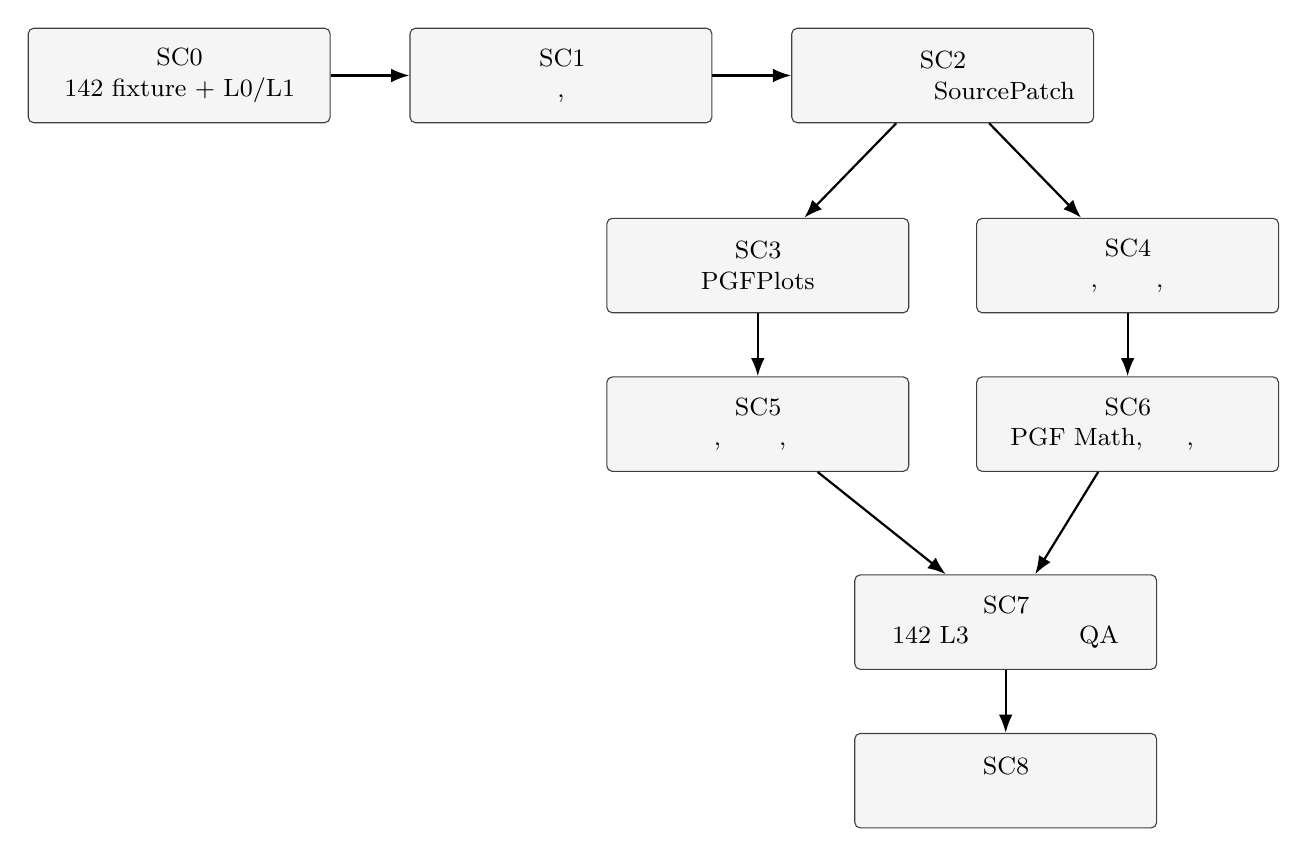
\begin{tikzpicture}[font=\small,>=Latex,major/.style={draw=black!75,fill=black!4,rounded corners=2pt,minimum height=12mm,align=center,text width=3.6cm},arr/.style={->,thick},node distance=8mm and 10mm]
\node[major] (qa) {SC0\\142 fixture + L0/L1};
\node[major,right=of qa] (session) {SC1\\Один рисунок, зависимости};
\node[major,right=of session] (scan) {SC2\\Распознаватель и SourcePatch};
\node[major,below left=12mm and -15mm of scan] (plot) {SC3\\PGFPlots};
\node[major,below right=12mm and -15mm of scan] (geo) {SC4\\Имена, заливки, слои};
\node[major,below=of plot] (ann) {SC5\\Углы, размеры, формы};
\node[major,below=of geo] (math) {SC6\\PGF Math, циклы, данные};
\node[major,below right=13mm and -7mm of ann] (accept) {SC7\\142 L3 и независимая QA};
\node[major,below=of accept] (release) {SC8\\Платформенный выпуск};
\draw[arr](qa)--(session);\draw[arr](session)--(scan);
\draw[arr](scan)--(plot);\draw[arr](scan)--(geo);
\draw[arr](plot)--(ann);\draw[arr](geo)--(math);
\draw[arr](ann)--(accept);\draw[arr](math)--(accept);
\draw[arr](accept)--(release);
\end{tikzpicture}
\caption{Критические зависимости функциональных этапов. R0 идёт отдельно.}
\end{figure}

\section{R0. Сохранить границы Windows 1.0}\label{r0.-ux441ux43eux445ux440ux430ux43dux438ux442ux44c-ux433ux440ux430ux43dux438ux446ux44b-windows-1.0}

\textbf{R0-01 / A+B+D+I.} Сверьте текущие W0--W4 по \texttt{docs/WINDOWS\_1\_0\_RELEASE\_CONTROL\_RU.md} и оригинальным артефактам. Не выводите новый функционал Scientific-142 в первый выпуск при действующей заморозке. Текущий \texttt{main} содержит работу с физическим DPI и W2. Принятие полного W2b, физической Windows 10 W3 и W4 должно быть отдельным решением.

\textbf{Критерий выхода:} существующая линия выпуска не зависит от разработки новых PGFPlots-адаптеров. Нельзя закрывать W2b или W3 на основе тестов корпуса L1.

\section{SC0. Зафиксировать тестовый корпус}\label{sc0.-ux437ux430ux444ux438ux43aux441ux438ux440ux43eux432ux430ux442ux44c-ux442ux435ux441ux442ux43eux432ux44bux439-ux43aux43eux440ux43fux443ux441}

\textbf{SC0-01 / D.} Импортируйте 100 исходников AK, 42 подготовленных Sarov, 74 локальных файла \texttt{.dat}, подключаемый \texttt{optics-common.tex} и 142 эталонных PDF. Проверяйте SHA-256 каждого файла. Не изменяйте авторские формулы при импортировании.

\textbf{SC0-02 / D.} Подключите \texttt{qa/validate\_corpus.py}. Проверьте 142 ID, пути, SHA, отсутствие Gnuplot и ровно один рисунок на файл. Добавьте негативный тест с повреждённым SHA.

\textbf{SC0-03 / A+D.} Выполните полный внешний XeLaTeX прогон. Сохраните код завершения, время, версию, число страниц, SHA исходника, SHA PDF и SHA лога. Снимайте \texttt{nullfont} как отдельный параметр.

\textbf{Результат SC0 в пакете:} завершено для L0/L1. Все 142 исходника собраны. Типографическая и ручная приёмка L1-V не завершена. Растровое сравнение L1-R в одном окружении выполнено для 142/142. Поддержка GUI L3 ещё не выполнялась.

\section{SC1. Один рисунок и локальные ресурсы}\label{sc1.-ux43eux434ux438ux43d-ux440ux438ux441ux443ux43dux43eux43a-ux438-ux43bux43eux43aux430ux43bux44cux43dux44bux435-ux440ux435ux441ux443ux440ux441ux44b}

\textbf{SC1-01 / A+B.} Добавьте \texttt{OneFigureSession} поверх текущего \texttt{Document}. Сеанс хранит один основной файл, ревизию, выделение, Undo и состояние PDF. Исключите модель нескольких активных холстов.

\textbf{SC1-02 / A.} Добавьте таблицу источников и контрольных сумм к существующему \texttt{ProjectDependencySnapshot}. Сохраняйте происхождение \texttt{.fls}. Определяйте изменения \texttt{\textbackslash{}input} и \texttt{.dat} без ложной актуальности.

\textbf{SC1-03 / B.} Покажите состояние «PDF актуален», «PDF устарел», «ошибка сборки». Обеспечьте правку и сохранение текущего файла. Не добавляйте галерею.

\textbf{SC1-04 / D.} Проверьте \texttt{AK-F6\_4}, \texttt{AK-F6\_5}, \texttt{AK-F14\_3}, \texttt{AK-F15\_1}, \texttt{AK-F21\_2}. Затем удалите тестовый \texttt{.dat} и подтвердите корректный отказ без изменения исходников.

\textbf{Выход:} один рисунок открывается с необходимыми локальными ресурсами; сборка и Undo не меняют их байты. Это ещё не доказывает визуальную правку всех конструкций.

\section{SC2. Распознавание, владение и SourcePatch}\label{sc2.-ux440ux430ux441ux43fux43eux437ux43dux430ux432ux430ux43dux438ux435-ux432ux43bux430ux434ux435ux43dux438ux435-ux438-sourcepatch}

\textbf{SC2-01 / C.} Реализуйте ограниченный TeX-сканер. Учитывайте UTF-8, скобки, группы, комментарии и области действия. Возвращайте диапазоны байтов и точность распознавания.

\textbf{SC2-02 / C.} Введите \texttt{RecognizedInstance} и \texttt{EditRequest}. Свяжите их с существующими \texttt{SourceTarget}, \texttt{SourcePatch} и общей ревизией. Откажитесь от правки при несовпадении исходника.

\textbf{SC2-03 / C+B.} Добавьте единый внутренний реестр адаптеров. Подключите параметры к существующему инспектору и F1. Сохраните \texttt{catalog-v1} для шести примитивов.

\textbf{SC2-04 / D.} Создайте негативные тесты: неизвестный макрос, вложенные группы, CRLF, кириллица, конфликт ревизий, перекрытие диапазонов, Undo после ручного изменения.

\textbf{Выход:} пользователь может изменить параметр распознанной чужой команды через GUI. Программа не изменяет соседние команды. Один Undo восстанавливает исходный SHA.

\section{SC3. PGFPlots: первый предметный адаптер}\label{sc3.-pgfplots-ux43fux435ux440ux432ux44bux439-ux43fux440ux435ux434ux43cux435ux442ux43dux44bux439-ux430ux434ux430ux43fux442ux435ux440}

\textbf{SC3-01 / C.} Реализуйте распознавание \texttt{axis}, его набора ключей и владения вложенными \texttt{\textbackslash{}addplot}. Сохраните \texttt{compat=1.17} из Sarov.

\textbf{SC3-02 / C.} Реализуйте изменения \texttt{domain}, \texttt{samples}, осевых границ, ticks, labels, размеров, цветов и типа маркера. Сохраняйте исходный синтаксис выражений.

\textbf{SC3-03 / B.} Добавьте инспектор Axis и инспектор Series. Показывайте исходные ключи и пояснения. Не создавайте внутренний движок графиков.

\textbf{SC3-04 / D.} Выполните GUI-прогоны \texttt{SV-001}, \texttt{SV-003}, \texttt{SV-009}, \texttt{SV-022}, \texttt{SV-029}. Каждый прогон включает исходный текст, правку, PDF, отмену и хэши.

\textbf{SC3-05 / C+D.} Добавьте \texttt{plot\ coordinates} и нативный TikZ plot формулы. Проверьте \texttt{SV-040} без Gnuplot и исходные AK-графики.

\textbf{Выход:} как минимум один реальный PGFPlots график можно изменять через обычный инспектор и вернуть к исходному виду. Профиль совместимости не меняется.

\section{SC4. Связанная геометрия и заливки}\label{sc4.-ux441ux432ux44fux437ux430ux43dux43dux430ux44f-ux433ux435ux43eux43cux435ux442ux440ux438ux44f-ux438-ux437ux430ux43bux438ux432ux43aux438}

\textbf{SC4-01 / C.} Реализуйте адаптер именованных путей. Свяжите \texttt{name\ path} и \texttt{name\ intersections} с исходными диапазонами. Не создавайте обратных координат по PDF.

\textbf{SC4-02 / C.} Реализуйте \texttt{fill\ between} с именами границ и параметрами \texttt{soft\ clip}. Не изменяйте точки границ при изменении стиля заливки.

\textbf{SC4-03 / B+C.} Реализуйте инспектор \texttt{patterns}, \texttt{patterns.meta}, \texttt{clip}, \texttt{pgf\ layers}. Для неподдержанного преобразования показывайте \texttt{OPAQUE}.

\textbf{SC4-04 / D.} Проверьте \texttt{SV-006}, \texttt{SV-007}, \texttt{SV-010}, \texttt{SV-027}, \texttt{SV-028}, \texttt{SV-039}. Зафиксируйте сохранность ссылок, слоёв и порядка команд.

\textbf{Выход:} пользователь изменяет заливку и исходный путь, не разрушая вычисляемые пересечения.

\section{SC5. Аннотации и специальные формы}\label{sc5.-ux430ux43dux43dux43eux442ux430ux446ux438ux438-ux438-ux441ux43fux435ux446ux438ux430ux43bux44cux43dux44bux435-ux444ux43eux440ux43cux44b}

\textbf{SC5-01 / C.} Добавьте адаптер \texttt{\textbackslash{}pic} с \texttt{angles} и \texttt{quotes}. Сохраняйте исходные вершины и текст метки.

\textbf{SC5-02 / C.} Добавьте адаптер \texttt{\textbackslash{}dimline} из \texttt{tikz-dimline}. Отдельно изменяйте отступ, выносные линии и положение подписи.

\textbf{SC5-03 / C+B.} Добавьте поддержанные ключи \texttt{shapes.geometric} и \texttt{shapes.arrows}. Покажите форму в инспекторе. Не превращайте узел в растровое изображение.

\textbf{SC5-04 / D.} Проверьте \texttt{SV-005}, \texttt{SV-035}, \texttt{SV-036}, \texttt{SV-038} и затронутые AK схемы.

\textbf{Выход:} инструментальные операции сохраняют точки привязки, метки и геометрические зазоры.

\section{SC6. Макросы, циклы и большой набор точек}\label{sc6.-ux43cux430ux43aux440ux43eux441ux44b-ux446ux438ux43aux43bux44b-ux438-ux431ux43eux43bux44cux448ux43eux439-ux43dux430ux431ux43eux440-ux442ux43eux447ux435ux43a}

\textbf{SC6-01 / C.} Добавьте безопасные свойства для \texttt{\textbackslash{}pgfmathsetmacro}.

Поддержите объявление функций \texttt{\textbackslash{}pgfmathdeclarefunction}. Сохраняйте исходное выражение и арность функции.

\textbf{SC6-02 / C.} Добавьте простое редактирование литеральных диапазонов \texttt{\textbackslash{}foreach}. Для непрозрачных циклов оставьте редактирование исходника.

\textbf{SC6-03 / A+B.} Ограничьте время распознавания и построения предварительных маркеров. Не обрабатывайте тысячи точек заново на каждом кадре интерфейса.

\textbf{SC6-04 / C+D.} Проверьте \texttt{SV-042}, \texttt{AK-F6\_4}, \texttt{AK-F6\_5}, графики \texttt{AK-F14\_3}, \texttt{AK-F15\_1}, \texttt{AK-F21\_2}. Сохраните SHA всех \texttt{.dat}.

\textbf{SC6-05 / A.} Проверьте отмену долгой сборки, зависимые входы, ограничение журнала и последний успешный PDF.

\textbf{Выход:} изменение одного литерального параметра приводит к пересчёту исходной фигуры TeX без потери зависимостей.

\section{SC7. Полная приёмка 142 рисунков}\label{sc7.-ux43fux43eux43bux43dux430ux44f-ux43fux440ux438ux451ux43cux43aux430-142-ux440ux438ux441ux443ux43dux43aux43eux432}

\textbf{SC7-01 / D.} Создайте 142 сценария настоящего GUI по \texttt{qa/GUI\_SCENARIOS.jsonl}. Для каждого выберите один реальный поддерживаемый параметр. Не принимайте пустую операцию или правку через текстовый редактор вместо GUI.

\textbf{SC7-02 / D.} Для каждого сценария сохраните SHA до правки, диапазон источника, текст SourcePatch, SHA после, PDF после, Undo, восстановленный SHA, лог компилятора и снимок GUI.

\textbf{SC7-03 / D.} Зафиксируйте уровень L2 для каждой конструкции, которую тестовый рисунок действительно использует. Неподдержанная конструкция должна оставаться отмеченной.

\textbf{SC7-04 / D.} Сравните PDF с эталоном на фиксированной версии TeX. Отдельно проверьте глифы и встраивание шрифтов. Не делайте единый «PASS» по одному коду завершения.

\textbf{SC7-05 / C+D.} Включите проверенные физические инварианты AK. Не выводите новые физические модели из скана.

\textbf{Выход:} 142/142 уникальных сценария L3 имеют наблюдаемые доказательства. Все семейства адаптеров, включённые в релиз, имеют отрицательные тесты. Допустимые незакрытые L4 случаи перечислены отдельно.

\section{SC8. Платформенная и релизная приёмка}\label{sc8.-ux43fux43bux430ux442ux444ux43eux440ux43cux435ux43dux43dux430ux44f-ux438-ux440ux435ux43bux438ux437ux43dux430ux44f-ux43fux440ux438ux451ux43cux43aux430}

\textbf{SC8-01 / A+D.} Запустите базовый L0/L1 в Linux CI. Привяжите результаты к точному source SHA.

\textbf{SC8-02 / A+D.} Выполните отдельный Windows-hosted MiKTeX прогон. Он не заменяет физическую Win10.

\textbf{SC8-03 / B+D.} Выполните реальные GUI-прогоны Windows 10 x64, включая 100/125/200 \%, шрифты, нативные диалоги, IME и внешний MiKTeX.

\textbf{SC8-04 / B+D.} Проведите отдельную физическую проверку macOS ARM64 M1/M4 перед заявлением поддержки этой платформы.

\textbf{SC8-05 / I.} Проверьте исходные артефакты, CI и протокол независимого QA. Примите или отклоните выпуск. Не ставьте релизный тег до завершения обязательных ворот.

\section{Группировка крупных работ}\label{ux433ux440ux443ux43fux43fux438ux440ux43eux432ux43aux430-ux43aux440ux443ux43fux43dux44bux445-ux440ux430ux431ux43eux442}

\begin{longtable}[]{@{}
  >{\raggedright\arraybackslash}p{(\columnwidth - 6\tabcolsep) * \real{0.2500}}
  >{\raggedright\arraybackslash}p{(\columnwidth - 6\tabcolsep) * \real{0.2500}}
  >{\raggedright\arraybackslash}p{(\columnwidth - 6\tabcolsep) * \real{0.2500}}
  >{\raggedright\arraybackslash}p{(\columnwidth - 6\tabcolsep) * \real{0.2500}}@{}}
\toprule\noalign{}
\begin{minipage}[b]{\linewidth}\raggedright
Этап
\end{minipage} & \begin{minipage}[b]{\linewidth}\raggedright
Основной выход
\end{minipage} & \begin{minipage}[b]{\linewidth}\raggedright
Зависимости
\end{minipage} & \begin{minipage}[b]{\linewidth}\raggedright
Ответственные
\end{minipage} \\
\midrule\noalign{}
\endhead
\bottomrule\noalign{}
\endlastfoot
SC0 & Корпус и компиляторный QA & Нет & D, A \\
SC1 & Один сеанс и ресурсы & SC0 & A, B \\
SC2 & Лексический распознаватель и правка & SC1 & C, B, D \\
SC3 & PGFPlots axis/series & SC2 & C, B \\
SC4 & Пересечения и заливки & SC2; частично SC3 & C, B \\
SC5 & Углы, размеры, формы & SC2 & C, B \\
SC6 & PGF Math, циклы, большие данные & SC2; совместно SC3/SC4 & A, C \\
SC7 & 142 L3 и визуальная приёмка & SC3--SC6 & D, I \\
SC8 & Платформенные испытания & SC7 & A, B, D, I \\
\end{longtable}

\textbf{Оценка трудоёмкости:} используйте размер пакета \texttt{S}, \texttt{M}, \texttt{L}, \texttt{XL} только для планирования загрузки. Не приравнивайте размер к обещанной дате. Самые сложные пакеты --- SC2, SC3, SC4 и SC7. Измерьте фактическую трудоёмкость на двух первых завершённых вертикалях. После этого уточните календарный план.

\section{Точные условия передачи между этапами}\label{ux442ux43eux447ux43dux44bux435-ux443ux441ux43bux43eux432ux438ux44f-ux43fux435ux440ux435ux434ux430ux447ux438-ux43cux435ux436ux434ux443-ux44dux442ux430ux43fux430ux43cux438}

\begin{itemize}
\tightlist
\item
  \textbf{SC0 → SC1:} 142 ID, 142 источника, 142 PDF, манифест, отрицательный тест целостности.
\item
  \textbf{SC1 → SC2:} один сеанс, рабочий граф зависимостей, обратимость исходника.
\item
  \textbf{SC2 → SC3/SC4:} принят contract \texttt{RecognizedInstance} и тест отказа при конфликте.
\item
  \textbf{SC3/SC4 → SC7:} реальные проверенные GUI-операции на именованных опорных рисунках.
\item
  \textbf{SC7 → SC8:} 142/142 L3 PASS по отдельным доказательствам; нет известных ошибок сохранности кода.
\item
  \textbf{SC8 → release:} отдельная физическая проверка каждой заявленной платформы и решение интегратора.
\end{itemize}

\section{Требования к PR и контрольным точкам}\label{ux442ux440ux435ux431ux43eux432ux430ux43dux438ux44f-ux43a-pr-ux438-ux43aux43eux43dux442ux440ux43eux43bux44cux43dux44bux43c-ux442ux43eux447ux43aux430ux43c}

Подготовьте отдельную ветку Scientific-142. Не объединяйте с незавершённой линией W2/W3 Windows 1.0. Группируйте изменения по рабочим пакетам. Один PR должен содержать законченную техническую вертикаль, а не отдельную механическую замену строки.

На проверке каждой ветки выполните \texttt{cargo\ fmt}, \texttt{cargo\ test\ -\/-locked}, применимые \texttt{clippy} проверки, корпус L0, целевые L1, негативные сценарии и unit-event GUI. Для заявленного GUI PASS дополнительно приложите настоящие скриншоты и PDF с известного окружения. Перед слиянием проверьте фактический SHA и оригинальные артефакты. Не запускайте непроверенный PR на постоянном Windows Server.

\chapter{Риски и решения}\label{ux440ux438ux441ux43aux438-ux438-ux440ux435ux448ux435ux43dux438ux44f}

\begin{longtable}[]{@{}
  >{\raggedright\arraybackslash}p{(\columnwidth - 4\tabcolsep) * \real{0.3333}}
  >{\raggedright\arraybackslash}p{(\columnwidth - 4\tabcolsep) * \real{0.3333}}
  >{\raggedright\arraybackslash}p{(\columnwidth - 4\tabcolsep) * \real{0.3333}}@{}}
\toprule\noalign{}
\begin{minipage}[b]{\linewidth}\raggedright
Риск
\end{minipage} & \begin{minipage}[b]{\linewidth}\raggedright
Влияние
\end{minipage} & \begin{minipage}[b]{\linewidth}\raggedright
Действие
\end{minipage} \\
\midrule\noalign{}
\endhead
\bottomrule\noalign{}
\endlastfoot
Неизвестный макрос меняет область действия & Повреждение исходника & Возвратите \texttt{OPAQUE} \\
Неверная привязка пересечения & Физически неправильный рисунок & Редактируйте только исходный путь \\
Несовместимая версия PGFPlots & Другие координаты и стили & Сохраняйте compat и версию \\
Отсутствует локальный \texttt{.dat} & Пустой график & Отметьте ошибку ресурса \\
Текст меняется после распознавания & Патч попадает в чужой диапазон & Проверяйте ревизию и старый текст \\
Изменился пользовательский шрифт & Неполный PDF & Отдельный glyph/font audit \\
Долгая формульная серия & Блокировка GUI & Выделите работу из UI-потока \\
Версия TeX меняет PDF & Ложный визуальный FAIL & Фиксируйте окружение и порог \\
Windows Server QA выдаёт SUCCESS & Ложный физический PASS & Проверяйте оригинальные PNG и HWND \\
Запуск TeX под HIGH Administrator & Выполнение недоверенного TeX & Покажите предупреждение; не называйте режим sandbox \\
Ложное сравнение PDF по хэшу & Разные метаданные PDF & Используйте страницу, растр, шрифты отдельно \\
\end{longtable}

\chapter{Матрица принятия результата}\label{ux43cux430ux442ux440ux438ux446ux430-ux43fux440ux438ux43dux44fux442ux438ux44f-ux440ux435ux437ux443ux43bux44cux442ux430ux442ux430}

Результат считается функционально готовым только после проверки следующих действий: выбор распознанного элемента, точная подсветка его исходника, изменение одного подтверждённого свойства через GUI, одна точечная правка, сборка правильного PDF, Undo, восстановление SHA-256 и отсутствие изменений в других данных.

Результат L1 не расширяет функциональный статус адаптера. Результат virtual egui event не заменяет физический desktop acceptance. Наличие подключённого пакета не означает, что инструмент поддерживает его визуальное редактирование.

\section{Контрольная таблица репрезентативных рисунков}\label{ux43aux43eux43dux442ux440ux43eux43bux44cux43dux430ux44f-ux442ux430ux431ux43bux438ux446ux430-ux440ux435ux43fux440ux435ux437ux435ux43dux442ux430ux442ux438ux432ux43dux44bux445-ux440ux438ux441ux443ux43dux43aux43eux432}

\begin{longtable}[]{@{}llll@{}}
\toprule\noalign{}
Тест & Исходник & Основная конструкция & Ворота \\
\midrule\noalign{}
\endhead
\bottomrule\noalign{}
\endlastfoot
T-001 & AK-F3\_1 & Формула и общее расстояние импульсов & L2/L3/L4 \\
T-002 & AK-F6\_4 & \texttt{\textbackslash{}input}, связная оптическая схема & L2/L3/L4 \\
T-003 & AK-F6\_5 & Отражение и параметр макроса & L2/L3/L4 \\
T-004 & AK-F14\_3 & Плотная кривая из \texttt{.dat} & L1/L3 \\
T-005 & AK-F15\_1 & Четыре кривые \texttt{plot\ file} & L1/L3 \\
T-006 & AK-F21\_2 & Шесть внешних файлов данных & L1/L3 \\
T-007 & SV-001 & \texttt{axis}, формула \texttt{gauss}, одна серия & L2/L3 \\
T-008 & SV-006 & Именованные пути, заливка & L2/L3 \\
T-009 & SV-010 & Вычисляемое пересечение & L2/L3 \\
T-010 & SV-027 & Перекрывающиеся заливки & L2/L3 \\
T-011 & SV-035 & Размерные элементы и формы & L2/L3 \\
T-012 & SV-038 & Угловые метки и подписи & L2/L3 \\
T-013 & SV-040 & Нативный TikZ plot без Gnuplot & L2/L3 \\
T-014 & SV-042 & PGF Math \texttt{gauss} и две серии & L2/L3 \\
\end{longtable}

\chapter{Проверка комплекта и источники}\label{ux43fux440ux43eux432ux435ux440ux43aux430-ux43aux43eux43cux43fux43bux435ux43aux442ux430-ux438-ux438ux441ux442ux43eux447ux43dux438ux43aux438}

\section{Воспроизводимость}\label{ux432ux43eux441ux43fux440ux43eux438ux437ux432ux43eux434ux438ux43cux43eux441ux442ux44c}

Данный пакет создаёт самостоятельный тестовый вход. Запуск \texttt{qa/compile\_suite.py} требует доступного внешнего XeLaTeX, установленных пакетов и шрифтов, упомянутых в исходниках. Содержимое пакета позволяет проверить SHA, запустить сборки и сопоставить результаты с 142 эталонными PDF без скачивания дополнительного материала рисунков.

\section{Основания архитектурного решения}\label{ux43eux441ux43dux43eux432ux430ux43dux438ux44f-ux430ux440ux445ux438ux442ux435ux43aux442ux443ux440ux43dux43eux433ux43e-ux440ux435ux448ux435ux43dux438ux44f}

\begin{itemize}
\tightlist
\item
  \href{https://github.com/i-shutov/tikzarium}{Текущий исходный репозиторий Tikzarium}.
\item
  \texttt{AGENTS.md}, \texttt{docs/ARCHITECTURE.md} и \texttt{docs/PRODUCT\_SPEC.md}.
\item
  \texttt{docs/WINDOWS\_1\_0\_RELEASE\_CONTROL\_RU.md} на зафиксированном Git SHA.
\item
  \texttt{crates/tikzarium-extensions/src/primitives.rs} и \texttt{primitive\_edit.rs}.
\item
  \texttt{crates/tikzarium-extensions/src/project\_imports.rs}.
\item
  \texttt{crates/tikzarium-app/src/tikz\_authoring.rs}, \texttt{tikz\_canvas.rs} и \texttt{studio\_ui.rs}.
\item
  Оригинальный корпус AK-100 от 07.11.2026. Шифр источника находится в манифесте.
\item
  Оригинальный Sarov \texttt{main.tex} и 42 отдельные подготовленные фигуры. Оба источника приведены в \texttt{QA\_MANIFEST.json}.
\item
  ГОСТ Р 58049-2017. В тексте использованы принципы УТР: прямой порядок слов, одно значение термина, однозначные требования, короткие команды и активный залог.
\end{itemize}

\textbf{Правило изменений:} если инженер выявил новый тип конструкции, добавьте новый ID требования, адаптер, положительный и отрицательный тест. Не объявляйте семейство поддержанным только по успешному XeLaTeX PDF.

\end{document}
